\chapter{Background}

\textit{Cos'è la vita? Da dove viene?} - Fino al XVIII secolo per rispondere a tale quesito si faceva riferimento alla fede nel vitalismo: l'esistenza di una forza vitale non subordinata a leggi della chimica e  della fisica.
Importanti svolte furono gli esperimenti, prima di Redi poi di Spallanzani, per dimostrare l'infondatezza della teoria della \textit{generazione spontanea}, secondo la quale la vita poteva generarsi da materia non vivente. Un'importante passo in avanti, in concomitanza con l'affermarsi della \textit{teoria cellulare}, fu il lavoro di Pasteur che stabilì un collegamento fra processi vitali e reazioni chimiche: per la conversione di zucchero in alcool (fermentazione) era necessaria la presenza di microorganismi.
\par Successivamente vi sono i lavori di Berthelot e Buchner (premio Nobel per la Chimica 1907), il quale dimostrò che era possibile ottenere la fermentazione in assenza di microorganismi, usando solamente sostanze estratte da essi.
Queste sostanze furono chiamate \textit{enzimi} (dal ted. Enzym, letteralmente «dentro il lievito»\supercite{enzimaTreccani}). Non si conosceva la loro natura chimica, si scoprì successivamente che tutti gli enzimi sono \textit{proteine} (dal greco «primario», «che occupa la prima posizione» \supercite{proteinaTreccani}).
Queste proteine agivano da catalizzatori: acceleravano le reazioni chimiche all'interno delle cellule senza cambiare la loro natura, quindi senza consumarsi, e senza entrare nei prodotti finali della reazione.

\par La scoperta degli enzimi portò ad un cambio di paradigma nel pensiero scientifico riguardo le origini della vita: veniva ora considerata come la conseguenza di numerosi processi chimici resi possibili dalle proteine \supercite{kessel_ben-tal_2018}.
I fondamenti del pensiero biologico si spostarono dal vitalismo al meccanicismo secondo il quale tutti i fenomeni naturali, vita compresa, sono governati dalle stesse leggi, sia per sostanze organiche che inorganiche.

\par L'inconorazione delle proteine a \textit{macromolecole più importanti della vita} si può legare ad un'altra svolta nel pensiero scientifico avvenuta nella seconda metà del XX secolo: la rivoluzione genetica. Le proteine sono ben più che "macchine molecolari": sono i prodotti primari dei geni e sono coinvolte nell'espressione dell'informazione genetica. È sullo sfondo di questa rivoluzione che l'informatica si è inserita all'interno del mondo della biologia.

\clearpage

\section{Background biologico}
\subsection{Organizzazione della vita: dagli atomi alle cellule}
Nonostante le grandi differenze in dimensione, dieta, riproduzione, morfologia, comportamento, vi è un tratto comune a tutti gli organismi viventi: sono composti di cellule. Tutte le cellule sono caratterizzate da una stupefacente somiglianza chimica poiché utilizzano molecole simili e hanno ereditato tutte le stesse \textit{intuizioni}\footnote{Il termine \textit{intuizione} è qui usato creativamente per indicare le soluzioni genetiche sviluppatesi e sopravvissute ad oggi. Non si intende attribuire intelligenza, pensiero o volontà all'evoluzione.} genetiche. Si pensa quindi vi sia un antenato comune a tutti i viventi: una cellula vissuta circa 3,5 miliardi di anni fa che conteneva un prototipo del macchinario universale della vita sulla Terra oggi \supercite{alberts2018essential}. \\

\par Prima di parlare di cellule è opportuno richiamare l'attenzione sulle strutture biologiche. L'organizzazione biologica si basa su una gerarchia di livelli strutturali \footnote{Questa sezione di background biologico si basa in larga parte su \fullcite{campbell_reece_2012}.}, ognuno dei quali poggia su un gradino sottostante: 

\begin{figure}[h]
	\centering
	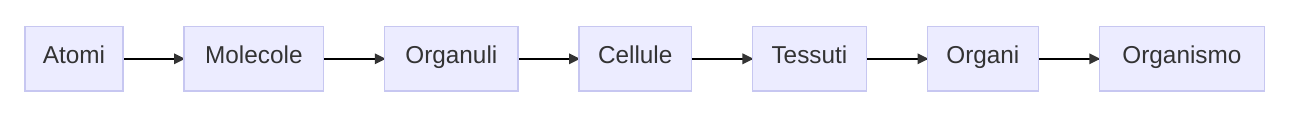
\includegraphics[scale=0.45] {images/strutture_biologiche.png}
\end{figure}


\par Tutta la materia è costituita da 94 elementi chimici in natura\supercite{elementiNaturaWiki} (tralasciando quindi gli altri 24 elementi sintetici). La materia vivente è composta per il 96\% da atomi di C, O, N, H (carbonio, ossigeno, azoto, idrogeno). Un atomo ha un nucleo composto da neutroni e protoni circondato da una nube di elettroni in rapido movimento. Il Dalton (Da) è l'unità della massa atomica, corrisponde al peso di un protone o neutrone: $1 Da = 1.66 \times 10^{-24}g$. Un elettrone pesa $0.0005 Da$. $1 \angstrom = 0.1nm$ e nonostante non sia un'unità di lunghezza appartenente al SI è molto utilizzata per le dimensioni di molecole, legami e atomi, il cui raggio varia da $0.25$ e $3 \angstrom$
Gli elettroni più esterni sono chiamati \textit{elettroni di valenza} e determinano il comportamento chimico di un atomo.

\par Lo scheletro delle molecole organiche è formato da catene carboniose, lunghe catene di atomi di carbonio legati fra loro da legami covalenti (il tipo di legame chimico più forte). Salendo di complessità si arriva alle macromolecole biologiche, fondamentali per le cellule: carboidrati, lipidi, acidi nucleici e proteine. I carboidrati sono combustibili cellulari e materiale da costruzione, i lipidi sono sia depositi di energia che i principali costituenti delle membrane cellulari, gli acidi nucleici permettono di codificare l'informazione genica e le proteine sono alla base delle funzioni vitali.\\

La cellula è la più piccola unità in grado di vivere. Per \textit{vivente} si intende un essere dotato di: organizzazione interna, metabolismo, omeostasi, interazione con l'ambiente, adattamento, crescita e riproduzione.

\par Le cellule hanno dimensioni che variano dai \textit{micrometri} ($\mu m$) ai $centimetri$ delle uova di rana, gallina o struzzo ai $metri$ di neuroni con lunghi assoni. In figura \ref{fig:cellule-dimensioni} si possono notare le diverse dimensioni di alcune cellule.

\begin{figure}[!h]
	\centering
	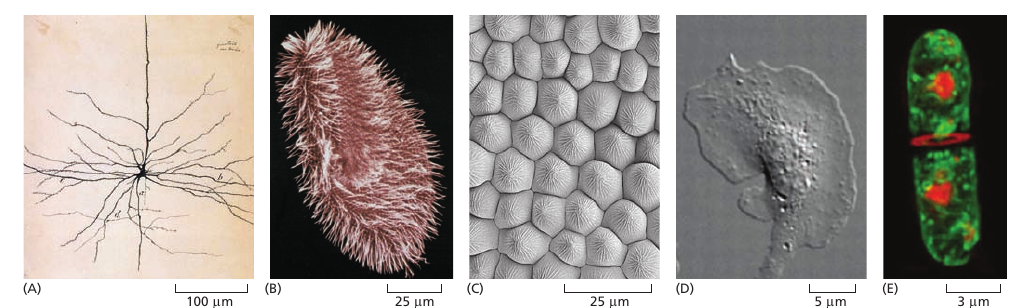
\includegraphics[scale=0.5] {images/cellule-dimensioni.png}
	\caption{(A) disegno di un neurone. (B) Paramecium. (C) superficie di un petalo di fiore di bocca di leone. (D) Macrofago. (E) Un lievito di fissione viene catturato nell'atto di divisione cellulare. Fonte: \cite{alberts2018essential}}
	\label{fig:cellule-dimensioni}
\end{figure}

\par È possibile dividere gli esseri viventi in due domini\footnote{Tale classificazione è soggetta a frequenti cambiamenti.}: \textit{procarioti} ed \textit{eucarioti}. Il primo include i due regni Bacteria e Archaea. Sono caratterizzati da cellule piccole, circa 1$\mu m$. Il secondo dominio include cinque regni: animali, piante, funghi, protisti e cromisti. Gli organismi eucarioti dispongono di cellule più grandi (circa 10-100 $\mu m$) dotate di compartimenti interni che separano le funzioni cellulari. La strutture tipiche di una cellula animale e di un neurone sono mostrate nelle seguenti figure:

\begin{figure}[!htb]
	\minipage{0.5\textwidth}
	\centering
	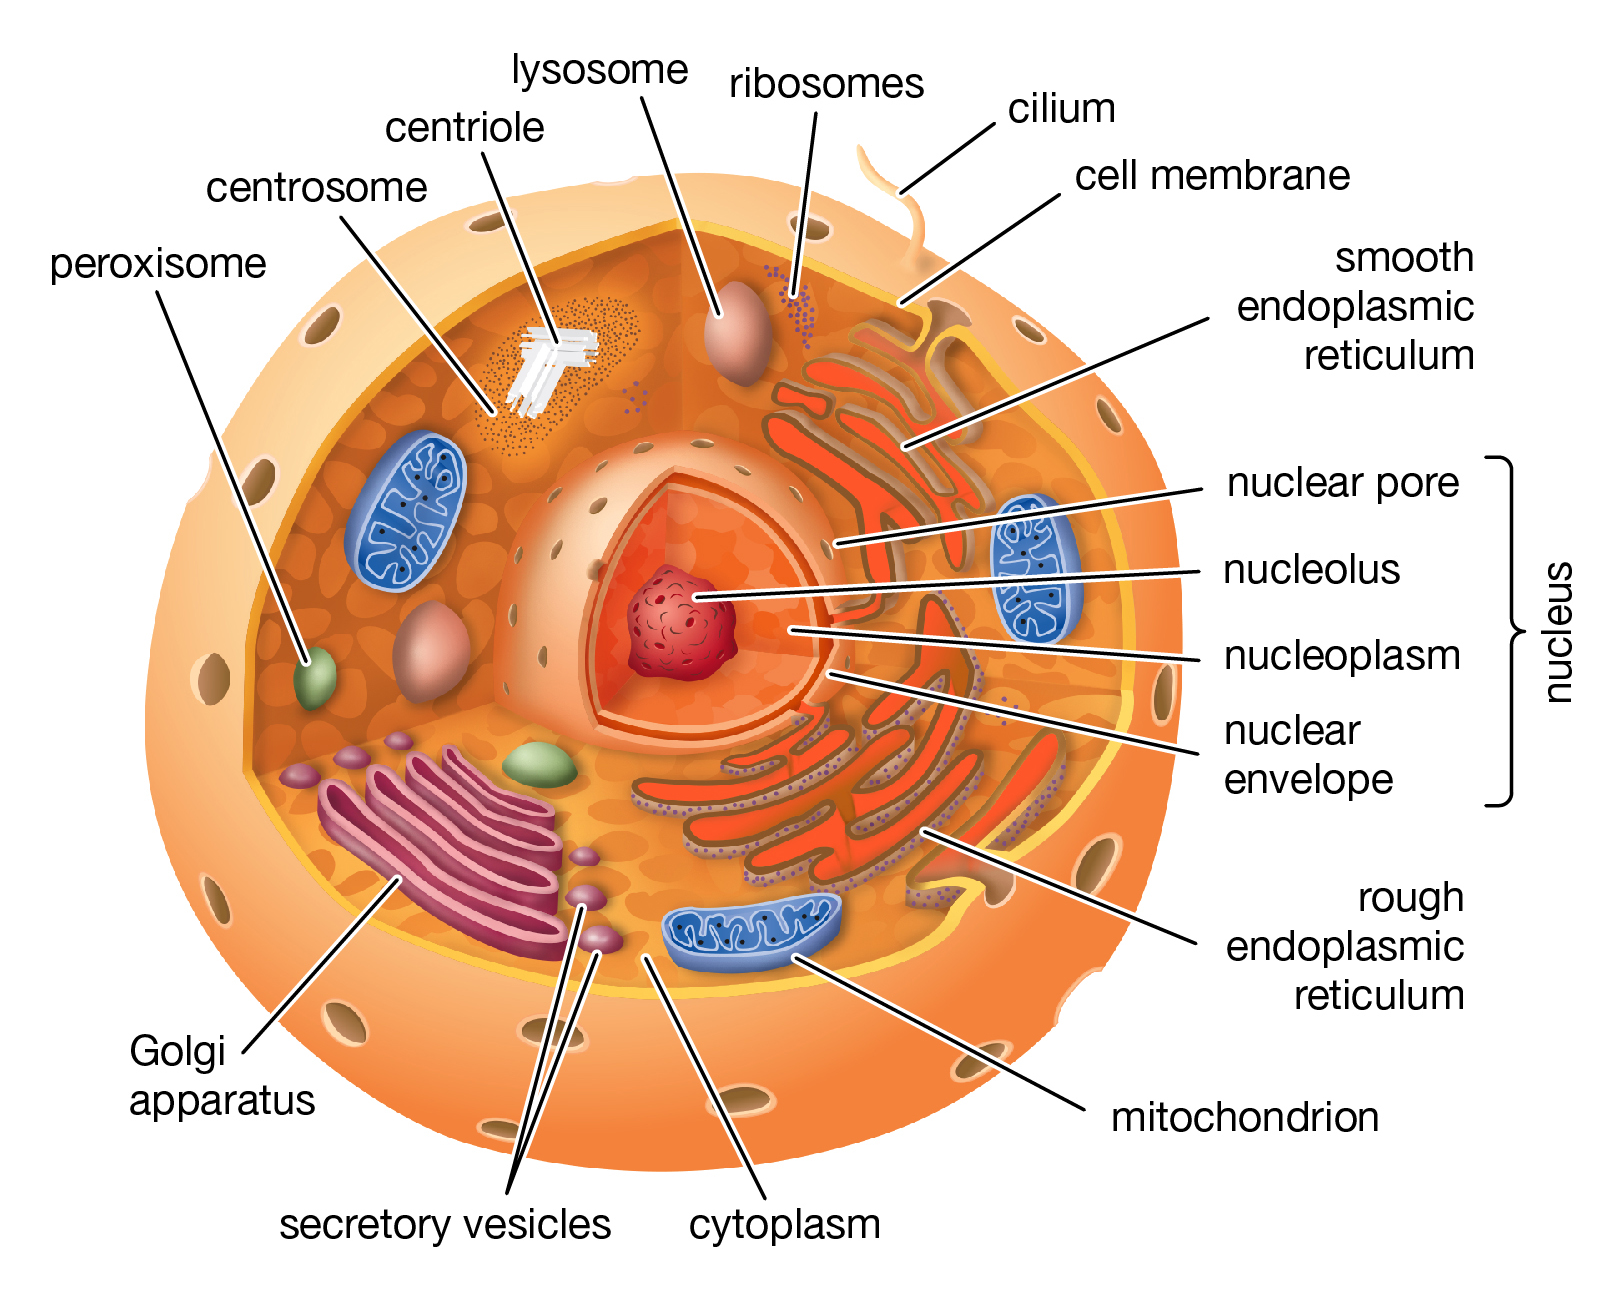
\includegraphics[scale=0.14]{images/cellula-eucariotica2.png}
	\caption{Cellula animale. Fonte: \cite{eukaryoteBritannica}}
	\label{fig:cellula-animale}
	\endminipage\hfill
	\minipage{0.5\textwidth}
	\centering
	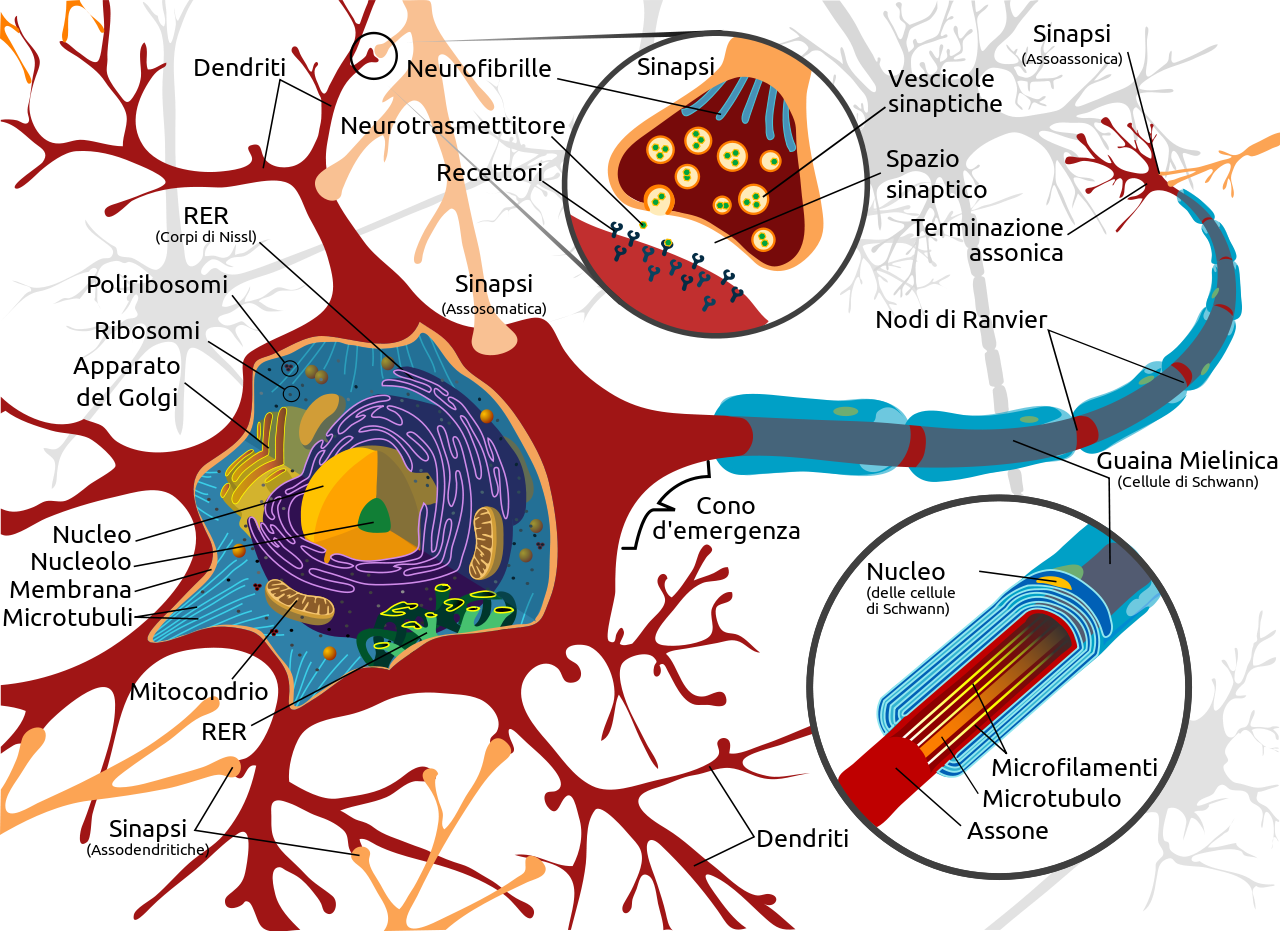
\includegraphics[scale=0.155]{images/neurone.png}
	\caption{Neurone. Fonte \cite{neuroneWiki}}
	\label{fig:neurone}
	\endminipage\hfill
\end{figure}

Una cellula eucariote animale è formata innanzitutto dalla membrana cellulare, un involucro costituito da un doppio strato fosfolipidico che permette alla cellula di avere il suo "spazio vitale" in quanto la separa dall'ambiente (spesso acquoso) circostante. È attraversata da piccoli pori che le permettono lo scambio di sostanze con l'esterno. Tutto ciò che si trova all'interno della cellula è immerso nel citoplasma, gel acquoso contenente grandi e piccole molecole. Il citosol è la parte del citoplasma non contenuta all'interno delle membrane intracellulari. Il volume totale delle cellule è composto da acqua per il 70\% circa. Vi è poi il citoscheletro che dà forma strutturale e permette in alcuni casi movimenti direzionati. 

\par Il primo organello di grande importanza è il reticolo endoplasmatico, formato da tubuli e cisterne e in comunicazione con l'involucro nucleare. È rugoso quando sono presenti ribosomi (sintetizzatori di proteine). È il componente della fabbrica cellulare che si occupa di attività e sintesi di molecole fondamentali per la sopravvivenza della cellula (sintesi di steroidi, metabolismo del glucosio, eliminazione di sostanze nocive). L'apparato del Golgi produce vescicole che si fondono poi con la membrana cellulare: è una centrale di smistamento per confezionare sostanze da esportare. I lisosomi sono il centro di degradazione e riciclo della cellula. Il mitocondrio è la centrale energetica della cellula, dove avviene la respirazione cellulare: utilizza ossigeno per bruciare molecole organiche degradate nel citoplasma come \textit{piruvato} e \textit{acetil-coenzima A} al fine di produrre energia che verrà immagazzinata sotto forma di ATP.

\par Infine è presente il nucleo, custode del DNA. È formato dall'involucro nucleare, cromatina e nucleolo. Il DNA nel nucleo è associato a delle proteine con cui forma un materiale fibroso chiamato cromatina, mostrandosi "sfilacciato" in modo da poter essere letto. Quando la cellula si riproduce la cromatina si condensa in strutture compatte e singole: i cromosomi. Il nucleolo non è provvisto di membrana e serve per la sintesi di RNA ribosomiale, cioè l'RNA che uscendo dai pori dell'involucro nucleare andrà nel citoplasma a formare i ribosomi. L'involucro nucleare possiede dei pori nucleari attraverso i quali possono transitare RNA e proteine, ma non DNA.

\par Il ciclo di vita delle cellule si basa su 4 fasi: crescita iniziale, sintesi del DNA, ulteriore crescita e mitosi (divisione cellulare). Le cellule dei mammiferi possono impiegare anche dei giorni per completare un ciclo di mitosi, mentre i lieviti solamente 90 minuti. Per questa ragione il lievito da fornaio (\textit{Saccharomyces cerevisiae}) è molto utilizzato in citologia e genetica: è uno degli organismi eucarioti modello\supercite{alberts2018essential} ed il suo genoma è stato il primo ad essere sequenziato completamente tra gli eucarioti \supercite{lievitoWiki}.

\par Le cellule hanno una durata di vita molto variabile, ad esempio alcuni organismi unicellulari come le spore possono vivere anche decenni, così come i nostri neuroni, mentre i globuli bianchi non sopravvivono oltre pochi giorni. \\

\par Gli strumenti utilizzati per indagare nel mondo microscopico riescono a mostrare dettagli che vanno dal limite di 200$nm$ del microscopio ottico (limite imposto dalla natura ondulatoria della luce) alla precisione di 1$nm$ del microscopio a trasmissione elettronica (che usa fasci di elettroni invece di fasci di luce ma di contro necessita di campioni molto fini):

\begin{figure}[!h]
	\centering
	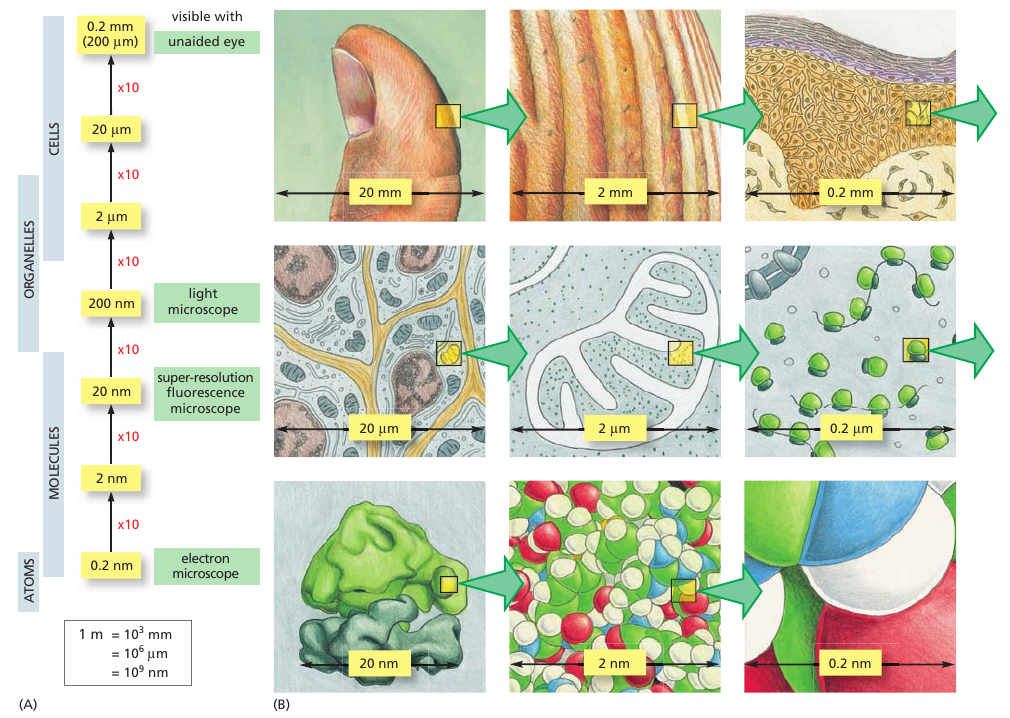
\includegraphics[scale=0.6]{images/grandezze.png}
	\caption{(A) Il grafico elenca le dimensioni dei livelli strutturali biologici, le unità di misura relative e gli strumenti necessari per visualizzarli. (B) Uno stesso dettaglio a varie scale di grandezza: pollice, pelle, cellule, mitocondrio, ribosomi, insieme di atomi che formano parte di una proteina. I dettagli molecolari sono oltre la potenza del microscopio elettronico. Fonte: \cite{alberts2018essential}}
	\label{fig:microscopi-grandezze}
\end{figure}

\subsection{Concetti fondamentali in biologia}

\begin{itemize}
	\item \textit{Proprietà emergenti }\\
			Ad ogni livello di indagine, ovvero passando da un livello della gerarchia strutturale al superiore, si palesano nuove proprietà non riconducibili ai livelli più semplici: le proprietà emergenti. Una singola molecola d'acqua non è né solida né liquida.
	\item \textit{Teoria cellulare} \\
			Le cellule rappresentano le unità strutturali e funzionali degli organismi.
	\item \textit{Geni} \\
			Il perpetuarsi della vita è possibile grazie alla trasmissione dei geni.
	\item \textit{Forma e funzione} \\
			Forma e funzione sono correlate a tutti i livelli biologici. Se le ali degli uccelli non fossero così come sono essi non potrebbero volare, se i mitocondri non avessero numero creste produrrebbero minori quantità di ATP, se i neuroni non avessero lunghi assoni non riuscirebbero a comunicare efficientemente e se i \textit{paramecium} non avessero le loro ciglia non potrebbero muoversi come sommergibili (vedi figura \ref{fig:cellule-dimensioni}B).
	\item \textit{Evoluzione} \\
			L'evoluzione rappresenta il tema centrale ed unificante della biologia, come si è già accennato sopra. Gli organismi sono sistemi aperti che interagiscono continuamente con l'ambiente, dotati di variabilità individuale e finalizzati alla competizione per la sopravvivenza. 
	\item \textit{Diversità e unità} \\
			Vi sono da 5 a 30 milioni di specie differenti eppure scendendo sempre di più nella struttura degli organismi si osserva una similitudine quasi sconcertante. Un esempio che ci riguarda è la somiglianza fra le ciglia di \textit{paramecium} e le ciglia di una cellula epiteliale delle vie aeree degli esseri umani: presentano la stessa sezione trasversale. Il codice genetico (le triplette) sono universali, gli amminoacidi si codificano nello stesso modo per tutti gli organismi. Diversità e unità della vita sulla Terra sono due facce della stessa medaglia. Il sequenziamento dei genomi e il loro confronto, basato su approcci informatici, ha rivelato una conservazione evoluzionistica, un'eredità comune: è possibile infatti scambiare geni omologhi codificanti proteine del ciclo di divisione cellulare fra uomini e lievito \supercite{alberts2018essential}: una cellula di lievito ha quindi tutto il macchinario molecolare necessario per leggere, interpretare e utilizzare il nostro codice genetico per la produzione di proteine umane funzionanti. Sono osservazioni simili che hanno guidato la direzione di alcune tecniche informatiche, anche per la predizione della struttura di proteine (come si vedrà successivamente).
			
\end{itemize}

\subsection{Dogma centrale della biologia}

Nel 1958 il premio Nobel Francis Crick introdusse il \textit{dogma} centrale della biologia, che allo stato attuale si può considerare come l'insieme dei principali meccanismi alla base dell'espressione genica. 

\begin{figure}[h]
	\centering
	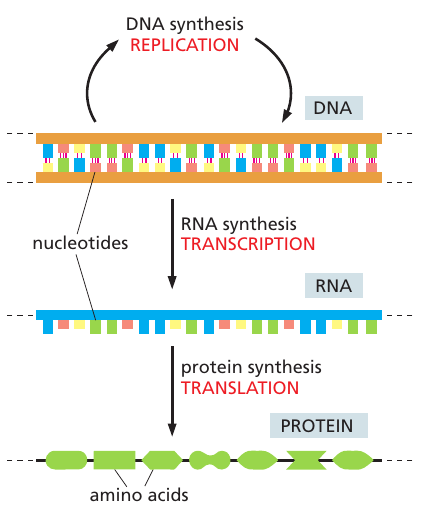
\includegraphics[scale=0.45]{images/central-dogma.png}
	\caption{Dogma centrale in biologia. Fonte \cite{alberts2018essential}}
	\label{fig:central-dogma}
\end{figure}

Il dogma descrive il flusso di informazione genetica: essa è conservata negli acidi nucleici DNA (RNA per alcuni virus) che possono essere duplicati, il DNA viene poi trascritto sotto forma di RNA e se codificante questo è poi tradotto in proteine, concepite come la forma operativa e terminale delle informazioni contenute nel genoma \supercite{dogma-wiki}.

\par Per avere una miglior panoramica del funzionamento di questo principio è importante approfondire la struttura del DNA (\textit{acido desossiribonucleico}). Il DNA è una molecola composta da due catene complementari che si avvolgono l'una intorno all'altra tramite legami idrogeno formando una doppia elica. Le catene sono chiamate filamenti e sono antiparalleli. Dal punto di vista chimico è un polimero di nucleotidi, dove ogni nucleotide è composto da una base azotata, uno zucchero pentoso (\textit{ribosio} nell'RNA e \textit{desossiribosio} nel DNA) e un gruppo fosfato (vedi figura \ref{fig:nucleotide}). Per ogni giro dell'elica vi sono 10 coppie di basi. La struttura a doppia elica consente un'agevole meccanismo di replicazione del DNA, coadiuvato dagli enzimi DNA polimerasi, primasi e DNA ligasi. Gli accoppiamenti seguono delle regole precise: GC, AT/AU, da una parte deve esserci una pirimidina (C, T) e dall'altra una purina (A,G):

\begin{figure}[!htb]
	\minipage{0.6\textwidth}
	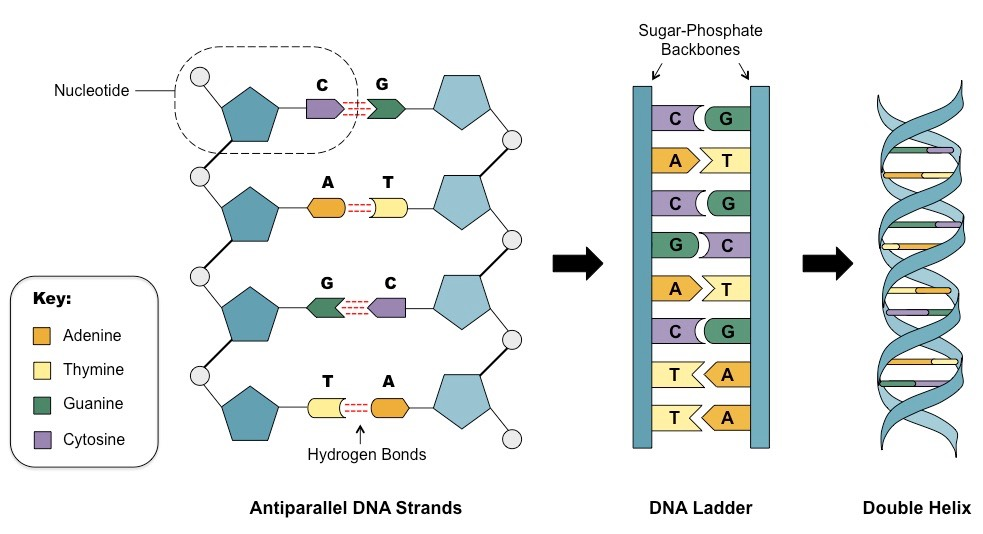
\includegraphics[scale=0.25]{images/double-stranded-dna_med.jpeg}
	\caption{struttura del DNA. Fonte: \cite{dna-image}}
	\label{fig:dna}
	\endminipage\hfill
	\minipage{0.4\textwidth}
	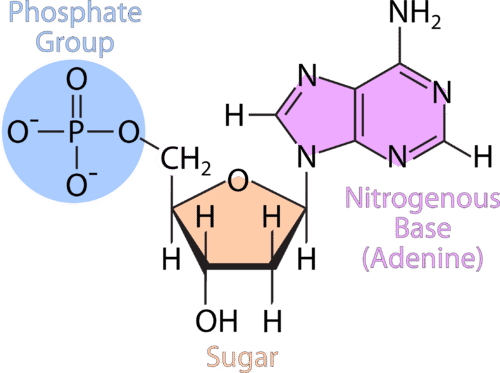
\includegraphics[scale=0.3]{images/nucleotide.png}
	\caption{Componenti di un nucleotide con Adenina per base azotata. Fonte \cite{introChimicaLibreTexts}}
	\label{fig:nucleotide}
	\endminipage\hfill
\end{figure}

Il \textit{gene} è l'unità elementare dell'informazione genetica e corrisponde al segmento di DNA (raramente di RNA) in grado di codificare la sequenza primaria di una proteina.  

 \begin{figure}[h]
	\centering
	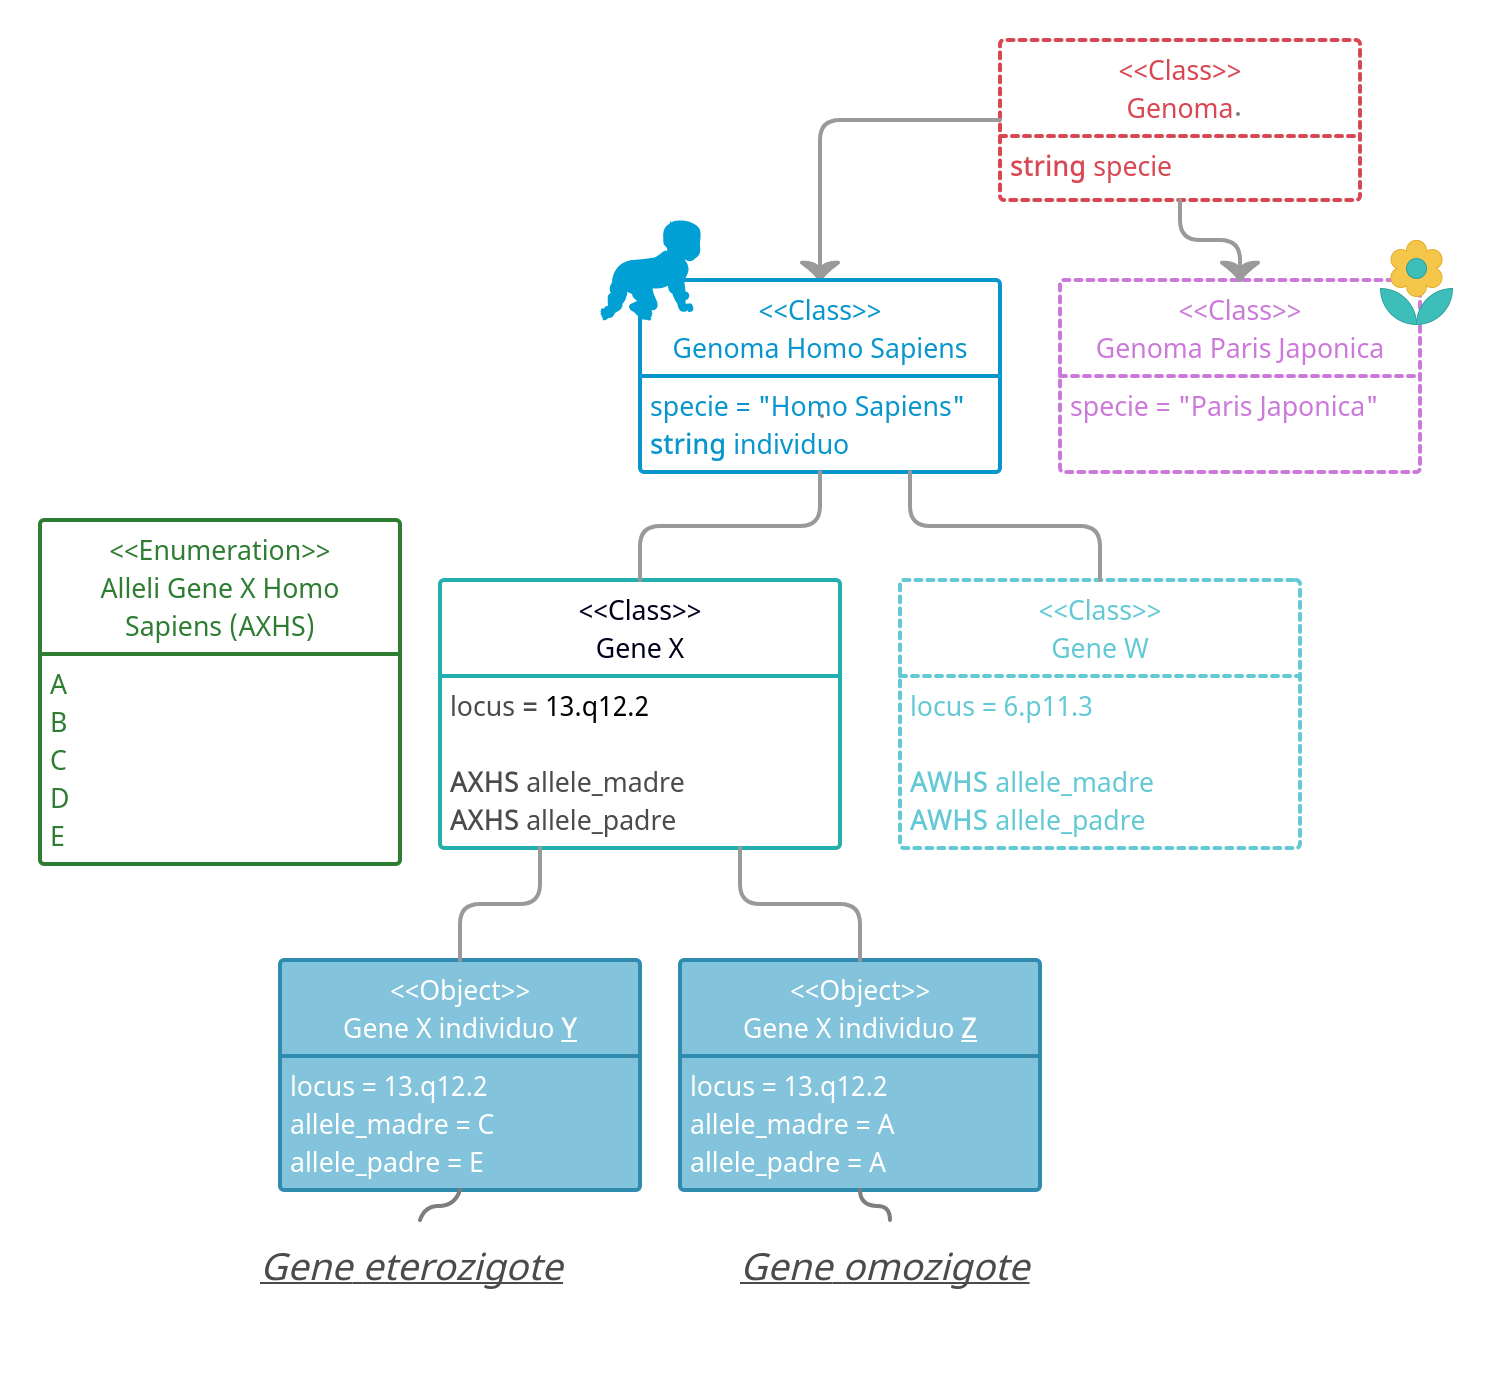
\includegraphics[scale=0.25]{images/alleli-uml.png}
	\caption{Schema UML di genoma e alleli in stile programmazione a oggetti. AXHS nella classe Gene X indica il tipo enumerazione definito accanto (diminutivo di \textbf{A}lleli Gene \textbf{X} \textbf{H}omo \textbf{S}apiens). AWHS nella classe gene W indica invece il tipo enumerazione che elenca i possibili alleli del gene W (non riportato). Ogni oggetto istanziato della classe Gene X avrà lo stesso locus genico e due possibili alleli. Creato su \href{https://creately.com}{creately.com}}
	\label{fig:alleli-uml}
\end{figure}

Geni che controllano un medesimo carattere (per esempio, il colore dei capelli) sono disposti sui cromosomi in \textit{loci} (plurale di locus genico, posizione) identici. I cromosomi omologhi sono cromosomi morfologicamente identici che presentano, in loci corrispondenti, gli stessi geni con le stesse informazioni. Ogni gene è presente in doppia coppia nelle cellule diploidi e può risultare pertanto omozigote od eterozigote.  Il termine omozigote si riferisce a un gene in cui l'informazione riportata dall'allele materno è identica a quella paterna, mentre in geni eterozigoti il contributo dell'allele materno e paterno è diverso: in questo caso la determinazione fenotipica è legata ai concetti di dominanza e recessività genetica. Lo stesso gene nella stessa specie può esistere in varie forme, con leggere differenze nella sequenza nucleotidica: si sta parlando degli \textit{alleli} del gene. Più precisamente l'insieme delle possibili versioni (1, 2 o più) dello stesso gene corrisponde ai suoi alleli. Un allele è quindi una delle versioni dello stesso gene nello stesso locus su un cromosoma.

\par Il \textit{genoma} indica il patrimonio complessivo del DNA di una cellula (compreso il DNA di altri organelli come mitocondri o cloroplasti). L'insieme di tutti i geni di un individuo determinano il suo \textit{genotipo} (quindi solo le regioni codificanti); relativamente a un gene il genotipo può anche indicare il corredo di alleli che l'organismo si trova a possedere (nell'uomo al massimo 2). Il \textit{fenotipo} indica invece l'insieme delle caratteristiche morfologiche e funzionali di un organismo, quali risultano dall'espressione del suo genotipo e dalle influenze ambientali. In un organismo, nonostante tutte le cellule condividano gli stessi geni, cellule diverse possono esprimere geni differenti (\textit{espressione genica}).

\begin{figure}[h]
	\centering
	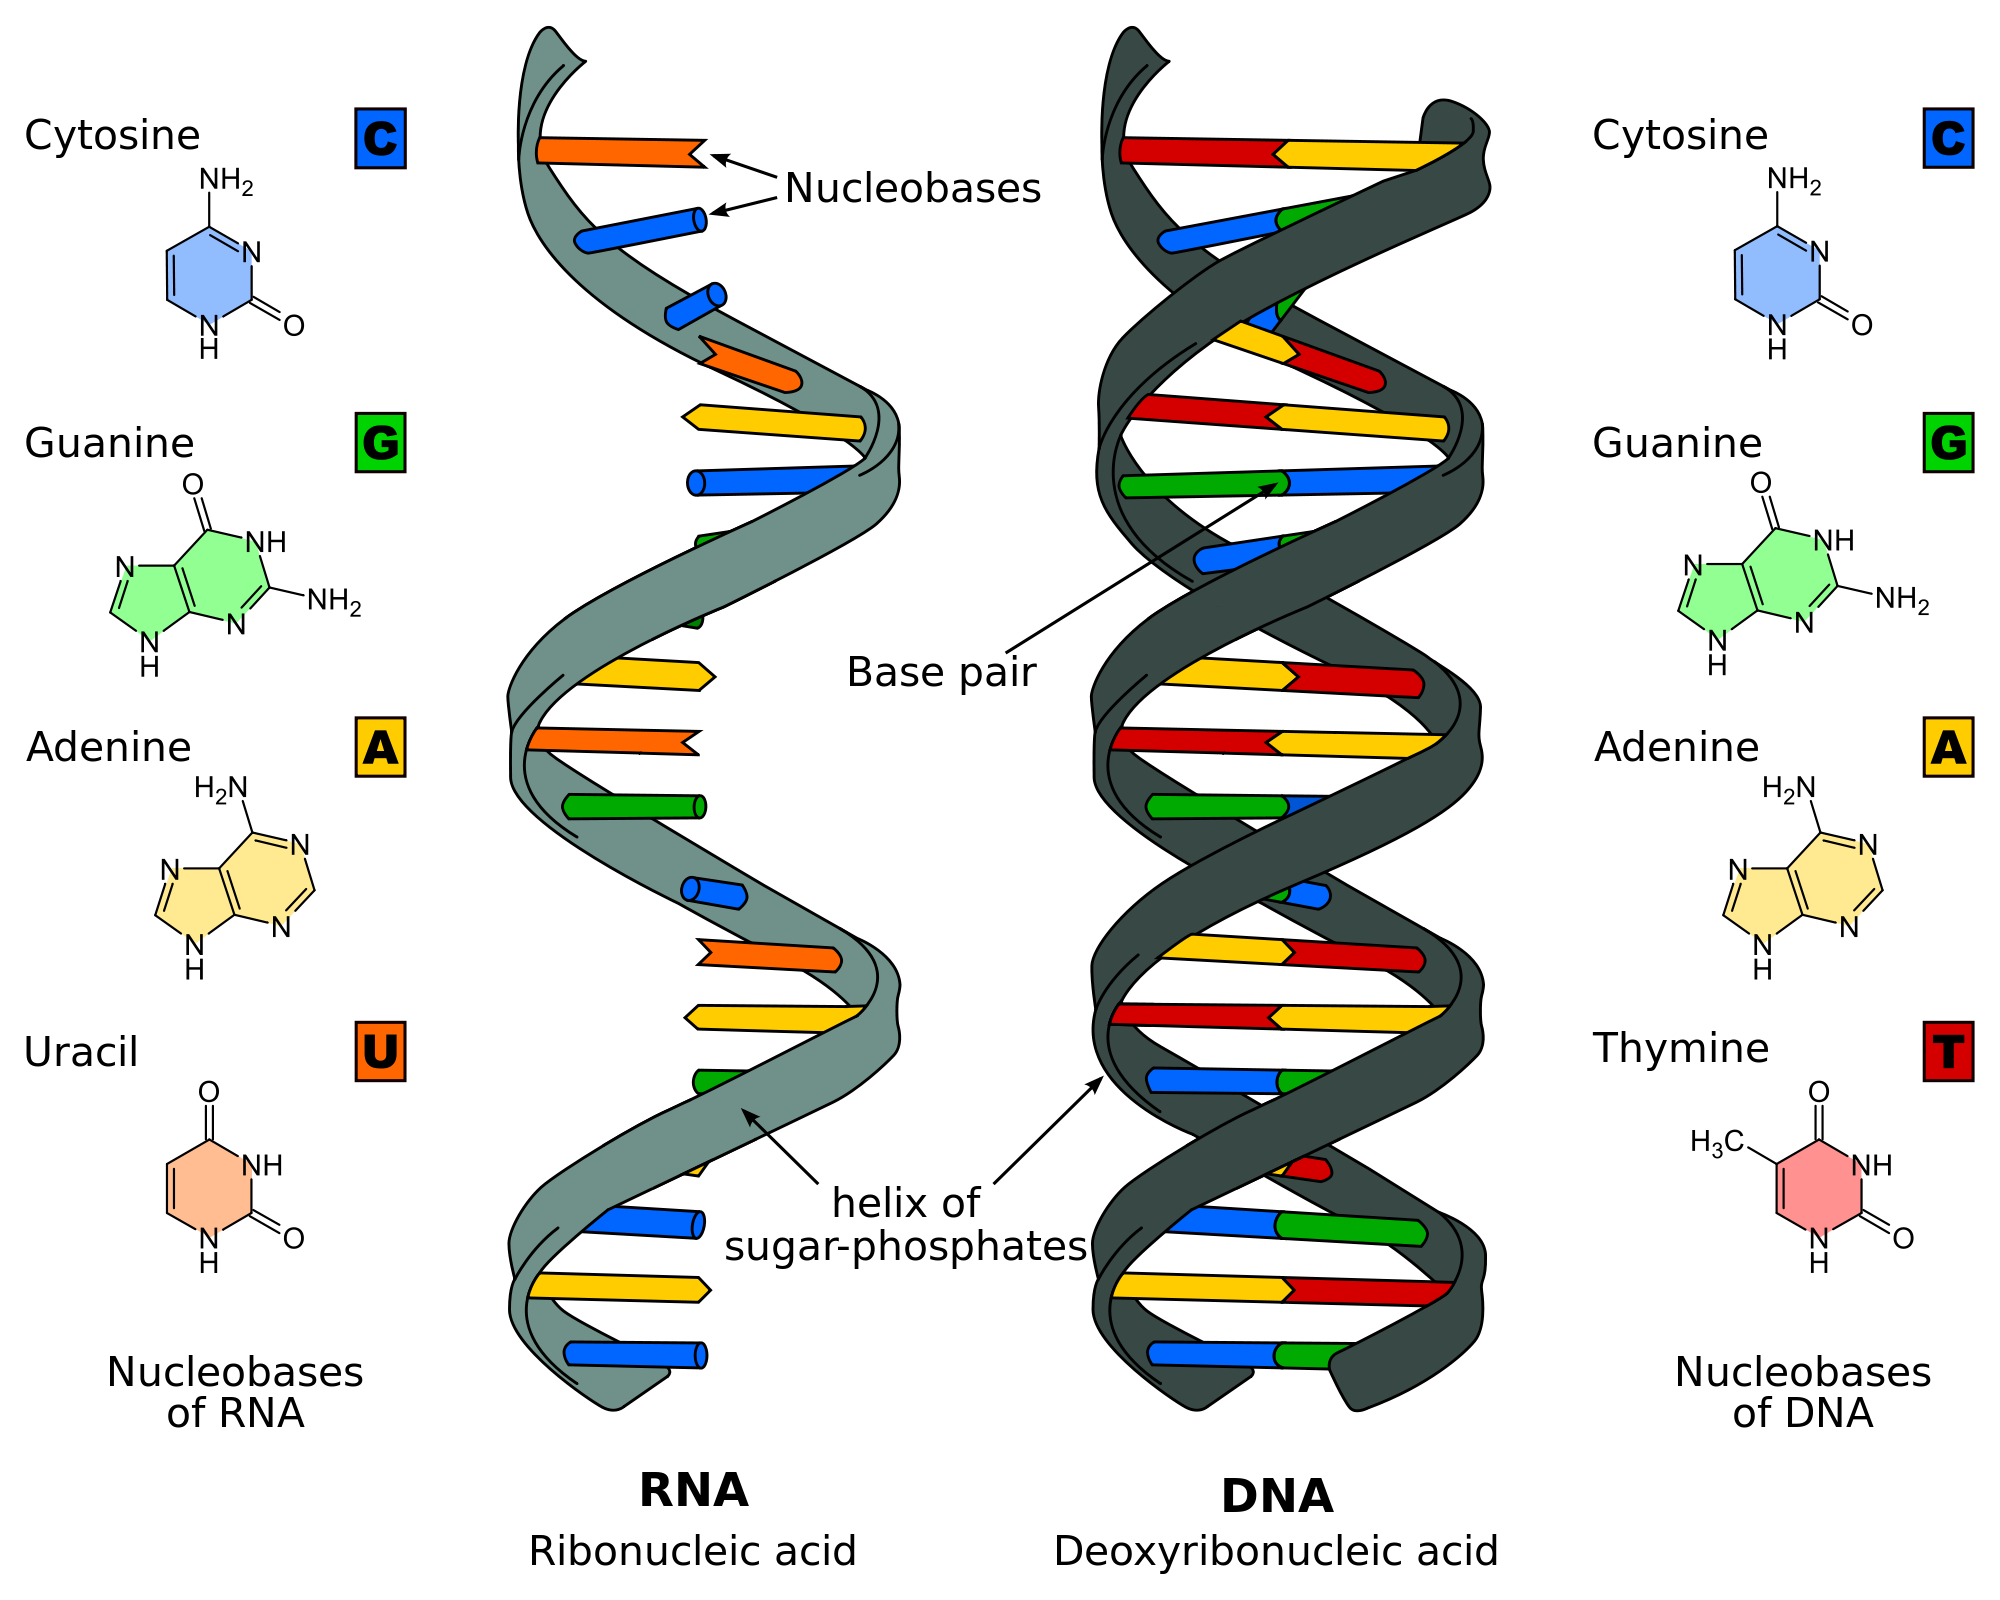
\includegraphics[scale=0.15]{images/dna-rna.png}
	\caption{Differenze fra RNA e DNA Fonte: \cite{dna-rna-image}}
	\label{fig:rna-dna-differenze}
\end{figure}

\par L'RNA (\textit{acido ribonucleico}) esiste in varie forme. Le differenze con il DNA sono mostrate nella figura \ref{fig:rna-dna-differenze}, si può notare che vi è un singolo filamento e che la base azotata timina è assente e al suo posto si trova la base uracile (U). Essendo ad un unico filamento può formare legami a idrogeno con sé stessa e assumere forme tridimensionali vantaggiose. Esistono vari tipi di RNA: 

\begin{itemize}
	\item mRNA, messaggero, contiene l'informazione per la sintesi delle proteine
	\item tRNA, di trasporto, necessario per la traduzione nei ribosomi
	\item rRNA, ribosomiale, entra nella struttura dei ribosomi
	\item snRNA, hnRNA
\end{itemize}

L'RNA catalitico o \textit{ribozima}, enzima ad RNA, è una molecola di RNA in grado di catalizzare una reazione chimica similmente agli enzimi. \\

\par Il DNA dell'uomo contiene $3\time10^{9}$ coppie di nucleotidi ($3.3Gbp$, \textit{gigabasepairs}), ha circa $21000$ geni codificanti e pesa $3.56pg$\footnote{In termini di massa è possibile convertire il numero di paia di basi azotate in \textit{picogrammi}, $1pg$=$0.978Gbp$, poiché una coppia di basi azotate pesa 650$Da$. Il peso del genoma umano è calcolabile come segue: $3.3\times10^{9}\times650\times1.66\times10^{-24}=3.56\times10^{-12}g$}: se il genoma umano venisse esteso in lunghezza sarebbe lungo 2,2 metri dato che ogni nucleotide è lungo $0.34nm$. Il batterio più semplice (\textit{Nasuia deltocephalinicola}) ha un genoma di 112Kb\supercite{nasuiaWiki} (circa $76\mu m$ in lunghezza) contenente 137 geni codificanti mentre il genoma maggiore ad oggi riportato è quello della pianta \textit{Paris Japonica} con 148.8Gbp\supercite{hidalgo2017there}, 50 volte quello dell'uomo (circa 100$m$ in lunghezza), tanto per avere una visione quantitativa della diversità genetica tra gli organismi.

\begin{figure}[!htb]
	\minipage{0.7\textwidth}
	\centering
	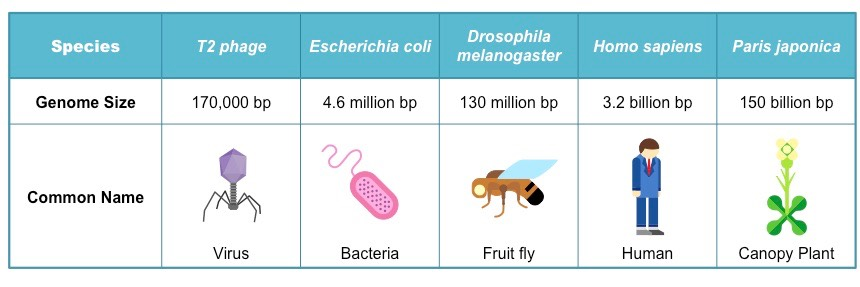
\includegraphics[scale=0.35]{images/genome-size-table_med.jpeg}
	\caption{Dimensioni del genoma di diverse specie a confronto. Fonte: \cite{genomeSizeBioNinja}}
	\label{fig:genome-size}
	\endminipage\hfill
	\minipage{0.28\textwidth}
	\centering
	
\includegraphics[scale=0.1]{images/Paris-japonica.jpg}
	\caption{Fiore di Paris Japonica. Fonte \cite{Pariswiki}}
	\label{fig:paris-japonica}
	\endminipage\hfill
\end{figure}

\subsection{Dai geni alle proteine}

Il codice genetico lavora a sequenze di codici di 3 lettere (es. "GAA" = Glutammato), questo perché si hanno a disposizione 4 lettere (le basi azotate) e si devono codificare i 20 diversi amminoacidi. Con 2 lettere avrei $4^{2}$ possibilità che non sono sufficienti a descrivere 20 informazioni diverse, si utilizzano pertanto 3 lettere anche se ciò causa ridondanza nei codici. Un amminoacido è quindi codificato da una tripletta: si parla di \textit{codice a triplette}. \\

\par Il primo passo consiste nella \textit{trascrizione}. Un filamento di DNA fa da stampo per la creazione di mRNA, il tutto esclusivamente tramite \textit{complementarità di forma}. Il DNA non viene aperto come una zip ma l'apertura, la trascrizione (compiuta dall'RNA polimerasi, soggetta a errori anche frequenti) e la chiusura della doppia elica avvengono di pari passo. Vi è un terminatore nel DNA per indicare la fine del gene. 

\par Le triplette nucleotidiche dell'mRNA sono dette \textit{codoni} e codificano un amminoacido. I codoni devono essere letti in direzione 5' -> 3'. La molecola di mRNA lascia il nucleo attraverso i pori nucleari. È importante osservare che non tutti i geni codificano proteine (lo stadio di trascrizione potrebbe risultare quello finale) e che il codice genetico è \textit{universale}, è condiviso dai batteri, piante, animali: per tutti la prolina si codifica in "CCG".

\par Negli eucarioti è presente un passaggio intermedio: la \textit{maturazione}, o fase di processamento. È composto da due sottofasi:
\begin{itemize}
	\item \textit{incapsulamento}, viene aggiunta una coda e un cappuccio alle due estremità al fine di proteggere l'mRNA dalla degradazione e per segnalare l'inizio ai ribosomi.
	\item \textit{splicing}, il DNA possiede lunghe sequenze nucleotidiche non codificanti, gli \textit{introni}. In questa fase vengono rimossi e gli \textit{esoni} (sequenze codificanti) vengono riunite insieme. È in questo modo che è possibile dare origini a sequenze primarie (delle proteine) diverse a partire da un unico gene.
\end{itemize}

\par L'ultimo passaggio è la \textit{traduzione}, attraverso la quale la cellula interpreta il messaggio genetico e polimerizza gli amminoacidi per costruire la relativa proteina. Il processo di traduzione è la transizione da un linguaggio a 4 lettere (basi azotate) ad un linguaggio a 20 lettere (amminoacidi). La traduzione viene realizzata dal tRNA, una sorta di adattatore da linguaggio \textit{genetico }a linguaggio \textit{amminoacidico}. Il tRNA è un acido nucleico a forma di L composto da circa 80 basi, a un'estremità vi è l'anticodone (interfaccia con il linguaggio genetico) e all'altra vi è il sito di legame con un singolo amminoacido. Il tRNA trasporta ai ribosomi uno specifico amminoacido contenuto nel citoplasma. Esiste di conseguenza uno specifico tipo di tRNA per ogni codone.

\begin{figure}[!htb]
	\minipage{0.5\textwidth}
	\centering
	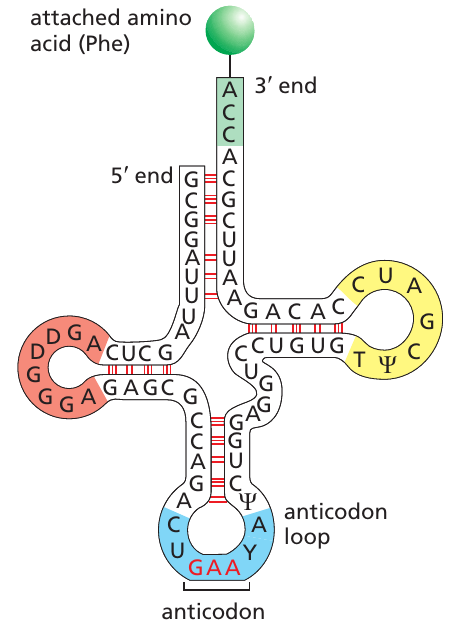
\includegraphics[scale=0.32]{images/tRNA.png}
	\caption{tRNA. Fonte \cite{alberts2018essential}}
	\label{fig:tRNA}
	\endminipage\hfill
	\minipage{0.5\textwidth}
	\centering
	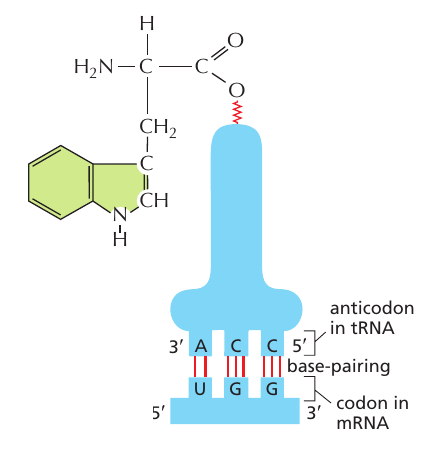
\includegraphics[scale=0.45]{images/tRNA-legame-traduzione.png}
	\caption{Traduzione: l'amminoacido triptofano (Trp) è codificato dal codone UGG nell'mRNA e si lega al tRNA tramite un legame energetico forte. Fonte: \cite{alberts2018essential}}
	\label{fig:tRNA-legame}
	\endminipage\hfill
\end{figure}

\par È interessante notare che il tRNA, proprio come le proteine, è caratterizzato dall'avere più strutture: quella primaria, costituita dalla sua sequenza nucleotidica, quella secondaria data dalla sua struttura a quadrifoglio e quella terziaria dovuta alla struttura tridimensionale a L. La differenza fra la struttura del tRNA e delle proteine sono gli elementi unitari: nel tRNA si tratta di nucleotidi mentre nelle proteine di amminoacidi.

\begin{figure}[h]
	\centering
	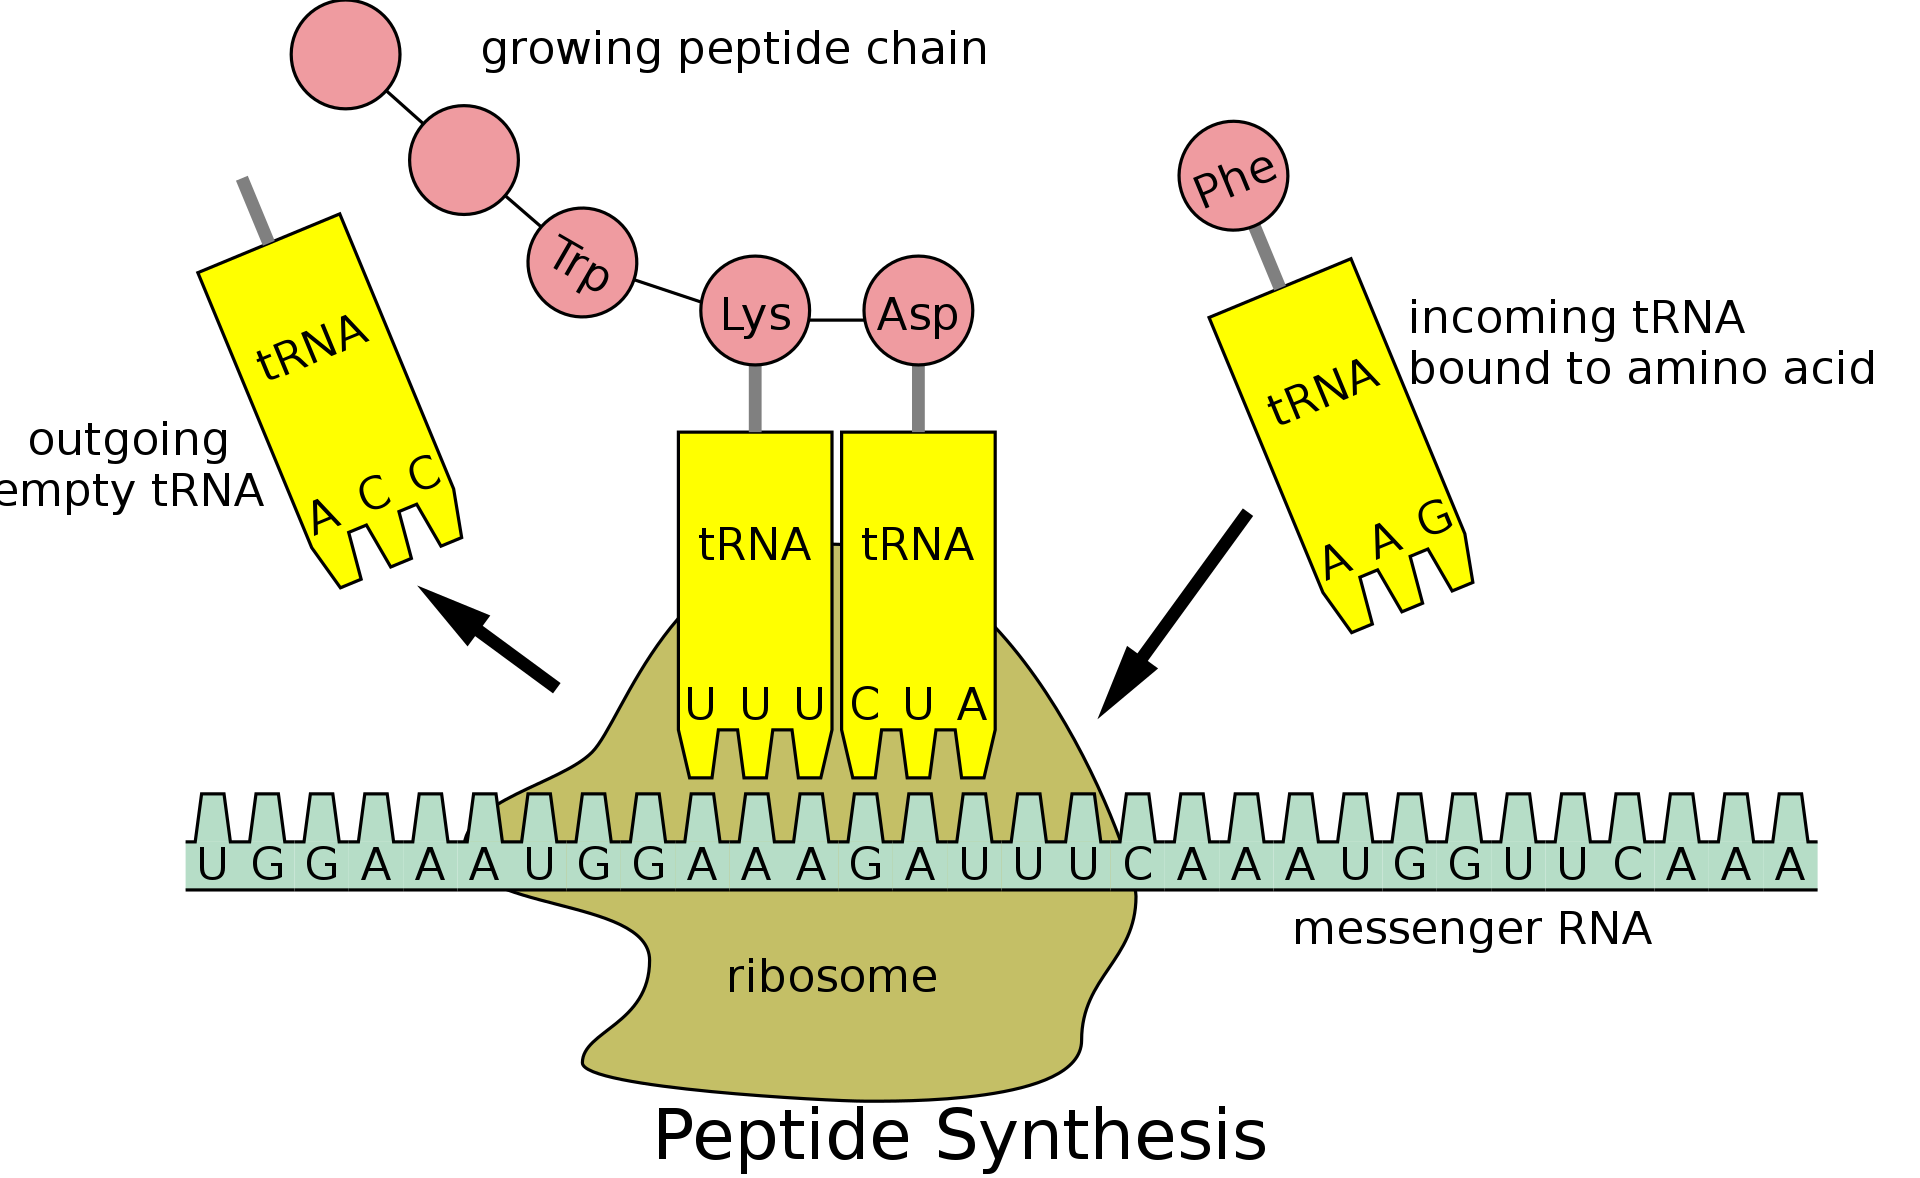
\includegraphics[scale=0.15]{images/traduzione.png}
	\caption{Traduzione, sintesi peptidica. Fonte: \cite{tRNAwiki}}
	\label{fig:traduzione}
\end{figure}

La traduzione comincia con il primo codone (AUG, che oltre a segnalare l'inizio codifica anche la metionina, vedi figura \ref{fig:codici-amminoacidi}) al quale si incastra nel ribosoma un tRNA avente il corrispondente amminoacido legato. Si formano legami idrogeno fra i nucleotidi. Arriva un secondo tRNA combaciante con il successivo codone. I due amminoacidi si trovano vicini e formano un legame peptidico. L'mRNA scorre così che si crei posto per nuovi tRNA, nel frattempo gli amminoacidi si legano fra loro e cominciano a formare la proteina. Il ripiegamento della proteina comincia già durante la sua biosintesi. Il processo termina quando si arriva ad un codone di stop (es. UAA). Per velocizzare il processo di sintesi ribosomiale questo viene parallelizzato: tanti \textit{poliribosomi} sono associati allo stesso mRNA attuando una rapida sintesi di copie multiple di un polipeptide a partire da un unico mRNA.

\begin{figure}[h]
	\centering
	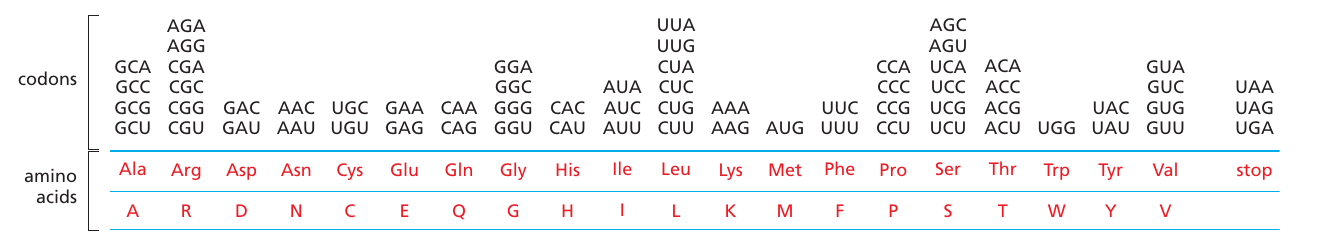
\includegraphics[scale=0.46]{images/codici-amminoacidi.png}
	\caption{Codici a tripletta degli amminoacidi. Fonte: \cite{alberts2018essential}}
	\label{fig:codici-amminoacidi}
\end{figure}

\subsection{Proteine: le macromolecole più importanti della vita}

Le proteine sono formate dall'unione di strutture più semplici: gli amminoacidi. Un polimero amminoacidico composto da meno di 50 amminoacidi è chiamato \textit{peptide}, se supera tale soglia \textit{polipeptide}. Una proteina può essere quindi sia un semplice peptide\footnote{Esempi di "semplici" peptidi che svolgono funzioni biologiche sono i \textit{neuropeptidi} che agiscono da neurotrasmettitore (ad es. endorfine) e \textit{ormoni} quali l'insulina, il glucagone e l'ossitocina, composta da soli 9 amminoacidi e implicata nelle contrazioni uterine e nella stimolazione dei dotti lattiferi delle mammelle.} che un singolo polipeptide o essere formata da più polipeptidi. La sequenza amminoacidica determina la struttura della proteina ed è proprio questo il collegamento fra il messaggio genetico nel DNA e la struttura tridimensionale che è associata alla sua funzione biologica. 

\par Un amminoacido è una molecola organica formata da un atomo di carbonio centrale chiamato $C_{\alpha}$ circondato da 4 componenti (vedi fig. \ref{fig:amminoacido}):
\begin{enumerate}
	\item un atomo di idrogeno
	\item un gruppo amminico ($\alpha-amino$), (-NH$_{2}$) in condizioni fisiologiche carico positivamente (-NH$_{3}^{+}$) 
	\item un gruppo carbossilico ($\alpha-carboxyl$), (-COOH) carico negativamente (-COO$^{-}$)
	\item un gruppo R, gruppo laterale chiamato anche \textit{residuo} che per sineddoche indica l'intero amminoacido una volta che questo si trova all'interno della catena proteica
\end{enumerate}

Vi sono circa 20 amminoacidi proteinogenici diversi (come si può vedere nella figura \ref{fig:codici-amminoacidi} o \ref{fig:amminoacidi-tipi}). Il gruppo laterale non partecipa alla catena della \textit{backbone} (spina dorsale) della proteina, resa stabile dai legami peptidici: rimane infatti libero di legarsi. È questo il "trucco" che consente alla proteina sia di ripiegarsi su sé stessa che di legarsi ad altre molecole. Gli amminoacidi possono essere polari, non polari, carichi (vedi figura \ref{fig:amminoacidi-tipi}) e causano differenti ripiegamenti della proteina. Di conseguenza ne influenzano la funzione, si pensi infatti al caso dell'anemia falciforme causata da 1 solo amminoacido di differenza: valina al posto del glutammato. La prima non è polare mentre il secondo è polare carico, ciò causa legami differenti, quindi ripiegamento differente e funzione biologica compromessa. 

\par Gli amminoacidi esistono in 2 configurazioni: L e D. Essi sono infatti molecole \textit{chirali}: le due configurazioni sono l'immagine speculare l'una dell'altra ma non sono sovrapponibili. Nella grande maggioranza degli organismi viventi le proteine sono composte solo da amminoacidi della serie L.

\begin{figure}[!htb]
	\minipage{0.45\textwidth}
	\centering
	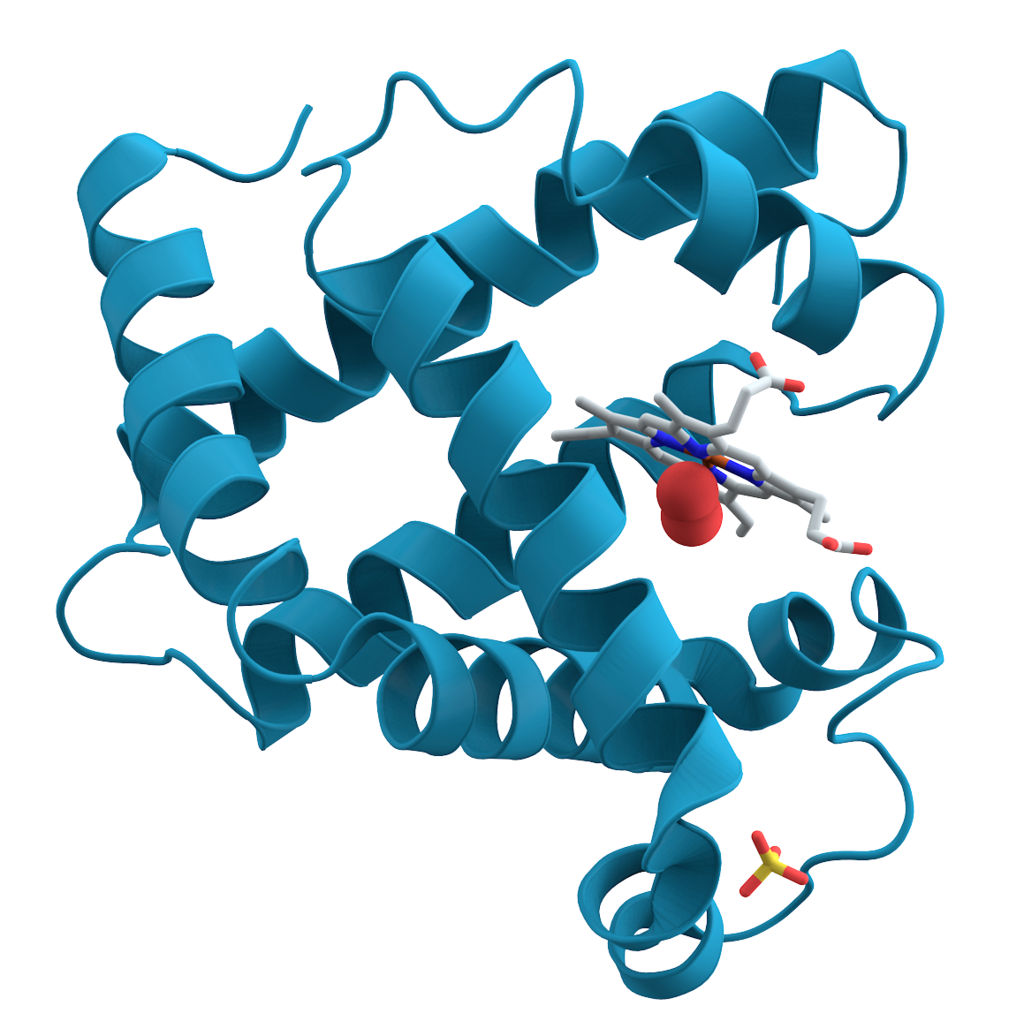
\includegraphics[scale=0.15]{images/mioglobina.png}
	\caption{Rappresentazione a nastro della struttura tridimensionale della mioglobina. È presente un gruppo hemo al quale è legata una molecola di ossigeno (rossa). Fonte: \cite{proteinWiki}}
	\label{fig:mioglobina}
	\endminipage\hfill
	\minipage{0.5\textwidth}
	\centering
	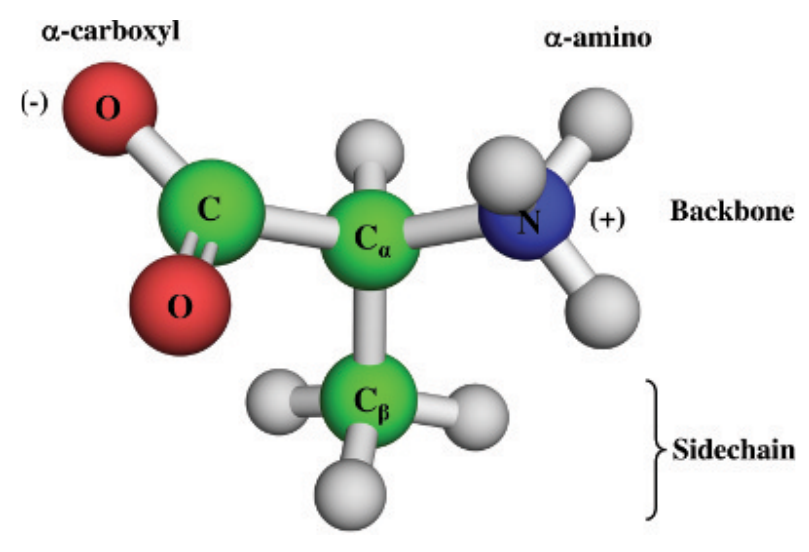
\includegraphics[scale=0.3]{images/amminoacido.png}
	\caption{Struttura principale degli amminoacidi. Fonte \cite{kessel_ben-tal_2018}}
	\label{fig:amminoacido}
	\endminipage\hfill
\end{figure}

\par Il legame peptidico è il legame che unisce tutti gli amminoacidi di una proteina: unisce il gruppo carbossilico di un amminoacido al gruppo amminico di un altro amminoacido. È un tipo di legame molto stabile, infatti l'emivita della backbone è di 400 anni a 25°C \supercite{alberts2018essential}. Il legame peptidico comporta l'eliminazione della carica degli ex gruppi \textit{amminico} e \textit{carbossilico}. 

\begin{figure}[!htb]
	\minipage{0.5\textwidth}
	\centering
	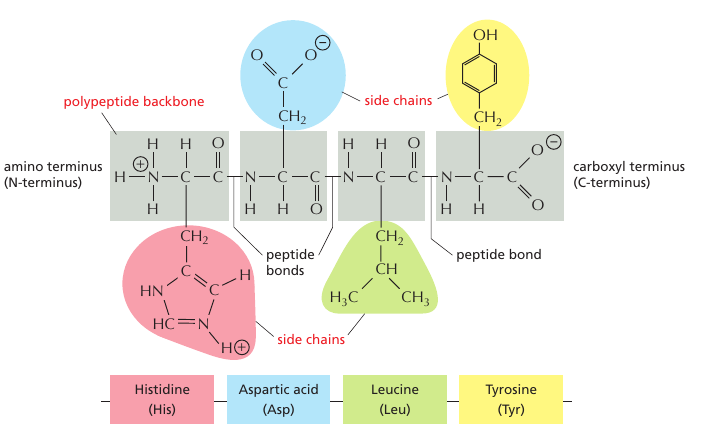
\includegraphics[scale=0.43]{images/protein-backbone.png}
	\caption{Backbone delle proteine. Fonte: \cite{alberts2018essential}}
	\label{fig:backbone}
	\endminipage\hfill
	\minipage{0.5\textwidth}
	\centering
	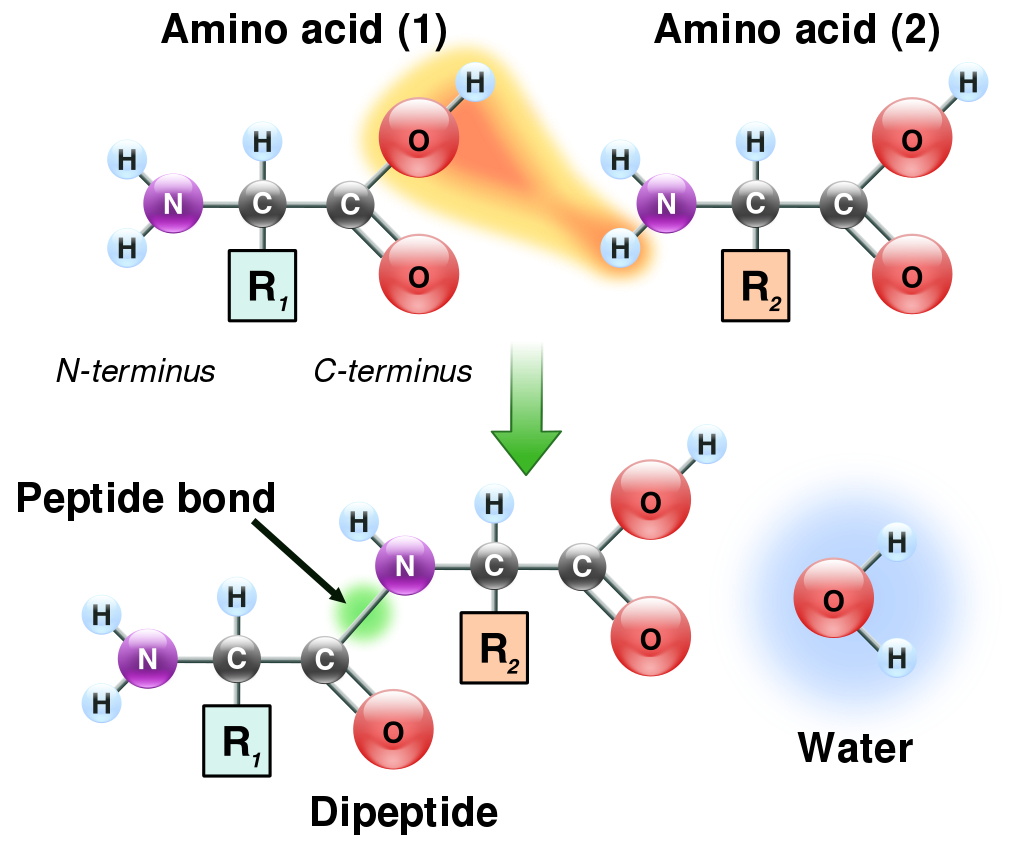
\includegraphics[scale=0.18]{images/peptide-bond.png}
	\caption{Legame peptidico. Fonte \cite{peptideBondWiki}}
	\label{fig:legame-peptidico}
	\endminipage\hfill
\end{figure}

Gli unici due residui elettricamente carichi rimasti in una proteina sono quelli alle due estremità (C-terminus ed N-terminus, vedi fig. \ref{fig:backbone}). È presente però un fenomeno che permette ai residui di interagire elettrostaticamente: la \textit{risonanza elettronica}. Gli elettroni dei legami possono estendersi su più atomi e permettere al residuo di assumere diverse configurazioni elettroniche. 

\par Nonostante gli amminoacidi siano solo 20, la varietà di proteine è elevatissima, in quanto gli amminoacidi si combinano tra loro in sequenze e quantità diverse. Dato un polipeptide di 100 amminoacidi si hanno $20^{100}$ possibili combinazioni. 

\begin{figure}[h]
	\centering
	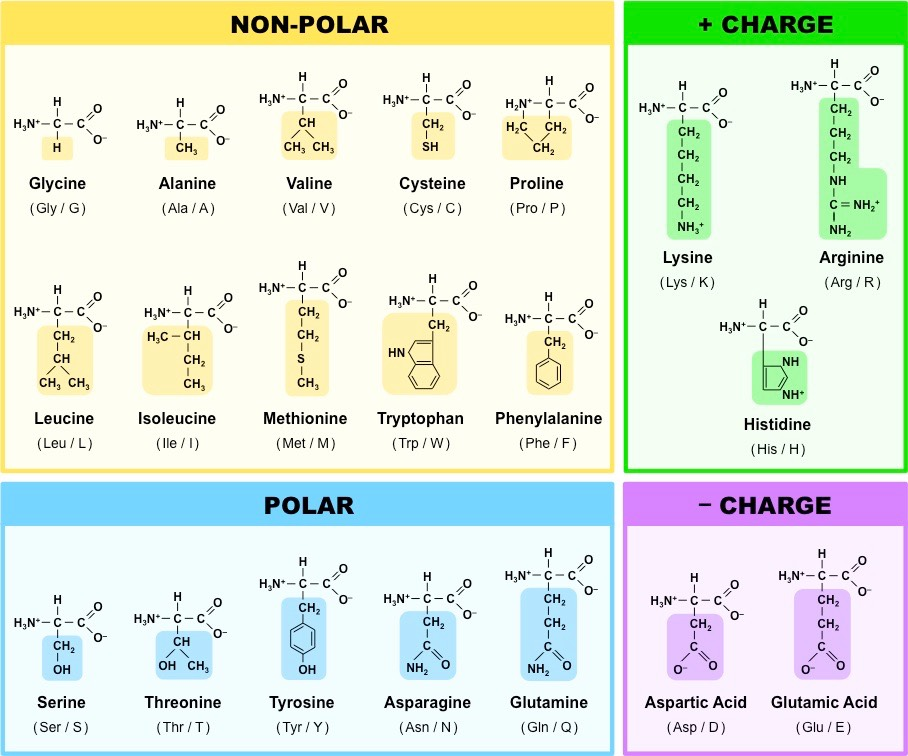
\includegraphics[scale=0.4]{images/aminoacid-tipi.jpeg}
	\caption{I 20 amminoacidi universali. Fonte: \cite{aminoacidTipi}}
	\label{fig:amminoacidi-tipi}
\end{figure}

È possibile in realtà parlare anche di altri amminoacidi e di derivati. La \textit{selenocisteina} è considerata il 21° amminoacido (così come la \textit{pirrolisina} il 22°). È stata scoperta per la prima volta nel 1986 ed è codificato dal codone UGA, normalmente un codone di stop, che tuttavia in presenza di un particolare segmento di mRNA viene interpretato come elemento costitutivo. La sua struttura è identica a quella della cisteina con una sola differenza: un atomo di selenio al posto di quello di zolfo. Esistono poi una serie di derivati dagli amminoacidi. Si può dire ad esempio che la \textit{tirosina} sia il precursore della \textit{dopamina, melanina e adrenalina}, il \textit{triptofano} di \textit{serotonina e melatonina }. Tipicamente questi derivati sono modificati dopo la traduzione nei ribosomi: la proteina in formazione viene modificata tramite legami covalenti da parte di enzimi e vengono a formarsi questi derivati.

\par Le proteine sono una classe di macromolecole con funzioni biologiche vitali, consentono infatti il funzionamento di ogni sistema vivente. Riusciamo a pensare, parlare, a digerire il cibo, a muoverci grazie alle proteine. Sono la base della vita cellulare e molecolare. 

\par Un tipo fondamentale di proteine sono gli enzimi, come accennato inizialmente. Una loro funzione importante è correlata alla digestione negli animali. Enzimi come le \textit{amilasi} e le \textit{proteasi }sono in grado di ridurre le macromolecole (nella fattispecie amido e proteine) in unità semplici (maltosio e amminoacidi), assorbibili dall'intestino.

\par Oltre agli enzimi ci sono tante altre proteine importanti. Uno degli esempi più noti è l'emoglobina, proteina animale adibita a trasportare ossigeno dai polmoni ai tessuti così come a riportare CO$_{2}$ ai polmoni. Una molecola di emoglobina è composta da 4 polipeptidi e contiene 4 atomi di ferro che le consentono di legare reversibilmente 4 molecole di ossigeno.

\begin{figure}[!htb]
	\minipage{0.45\textwidth}
	\centering
	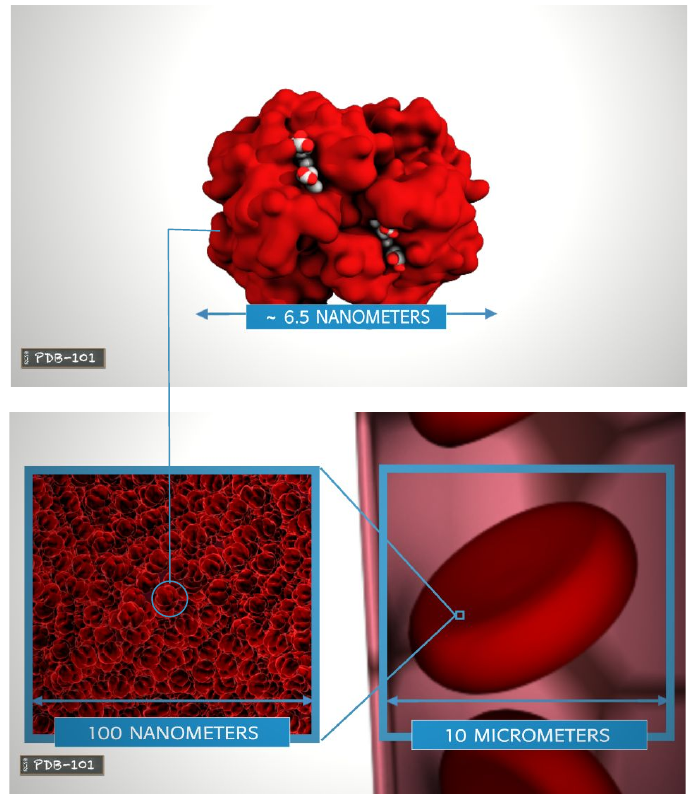
\includegraphics[scale=0.38]{images/emoglobina-dimensioni.png}
	\caption{Emoglobina in diverse scale. Rappresentazione a superficie. Un globulo rosso contiene circa 280 milioni di molecole di emoglobina, per cui può portare più di 1 miliardo di molecole di ossigeno per volta. Fonte: \cite{ProteinRCSB}}
	\label{fig:emoglobina-dimensioni}
	\endminipage\hfill
	\minipage{0.5\textwidth}
	\centering
	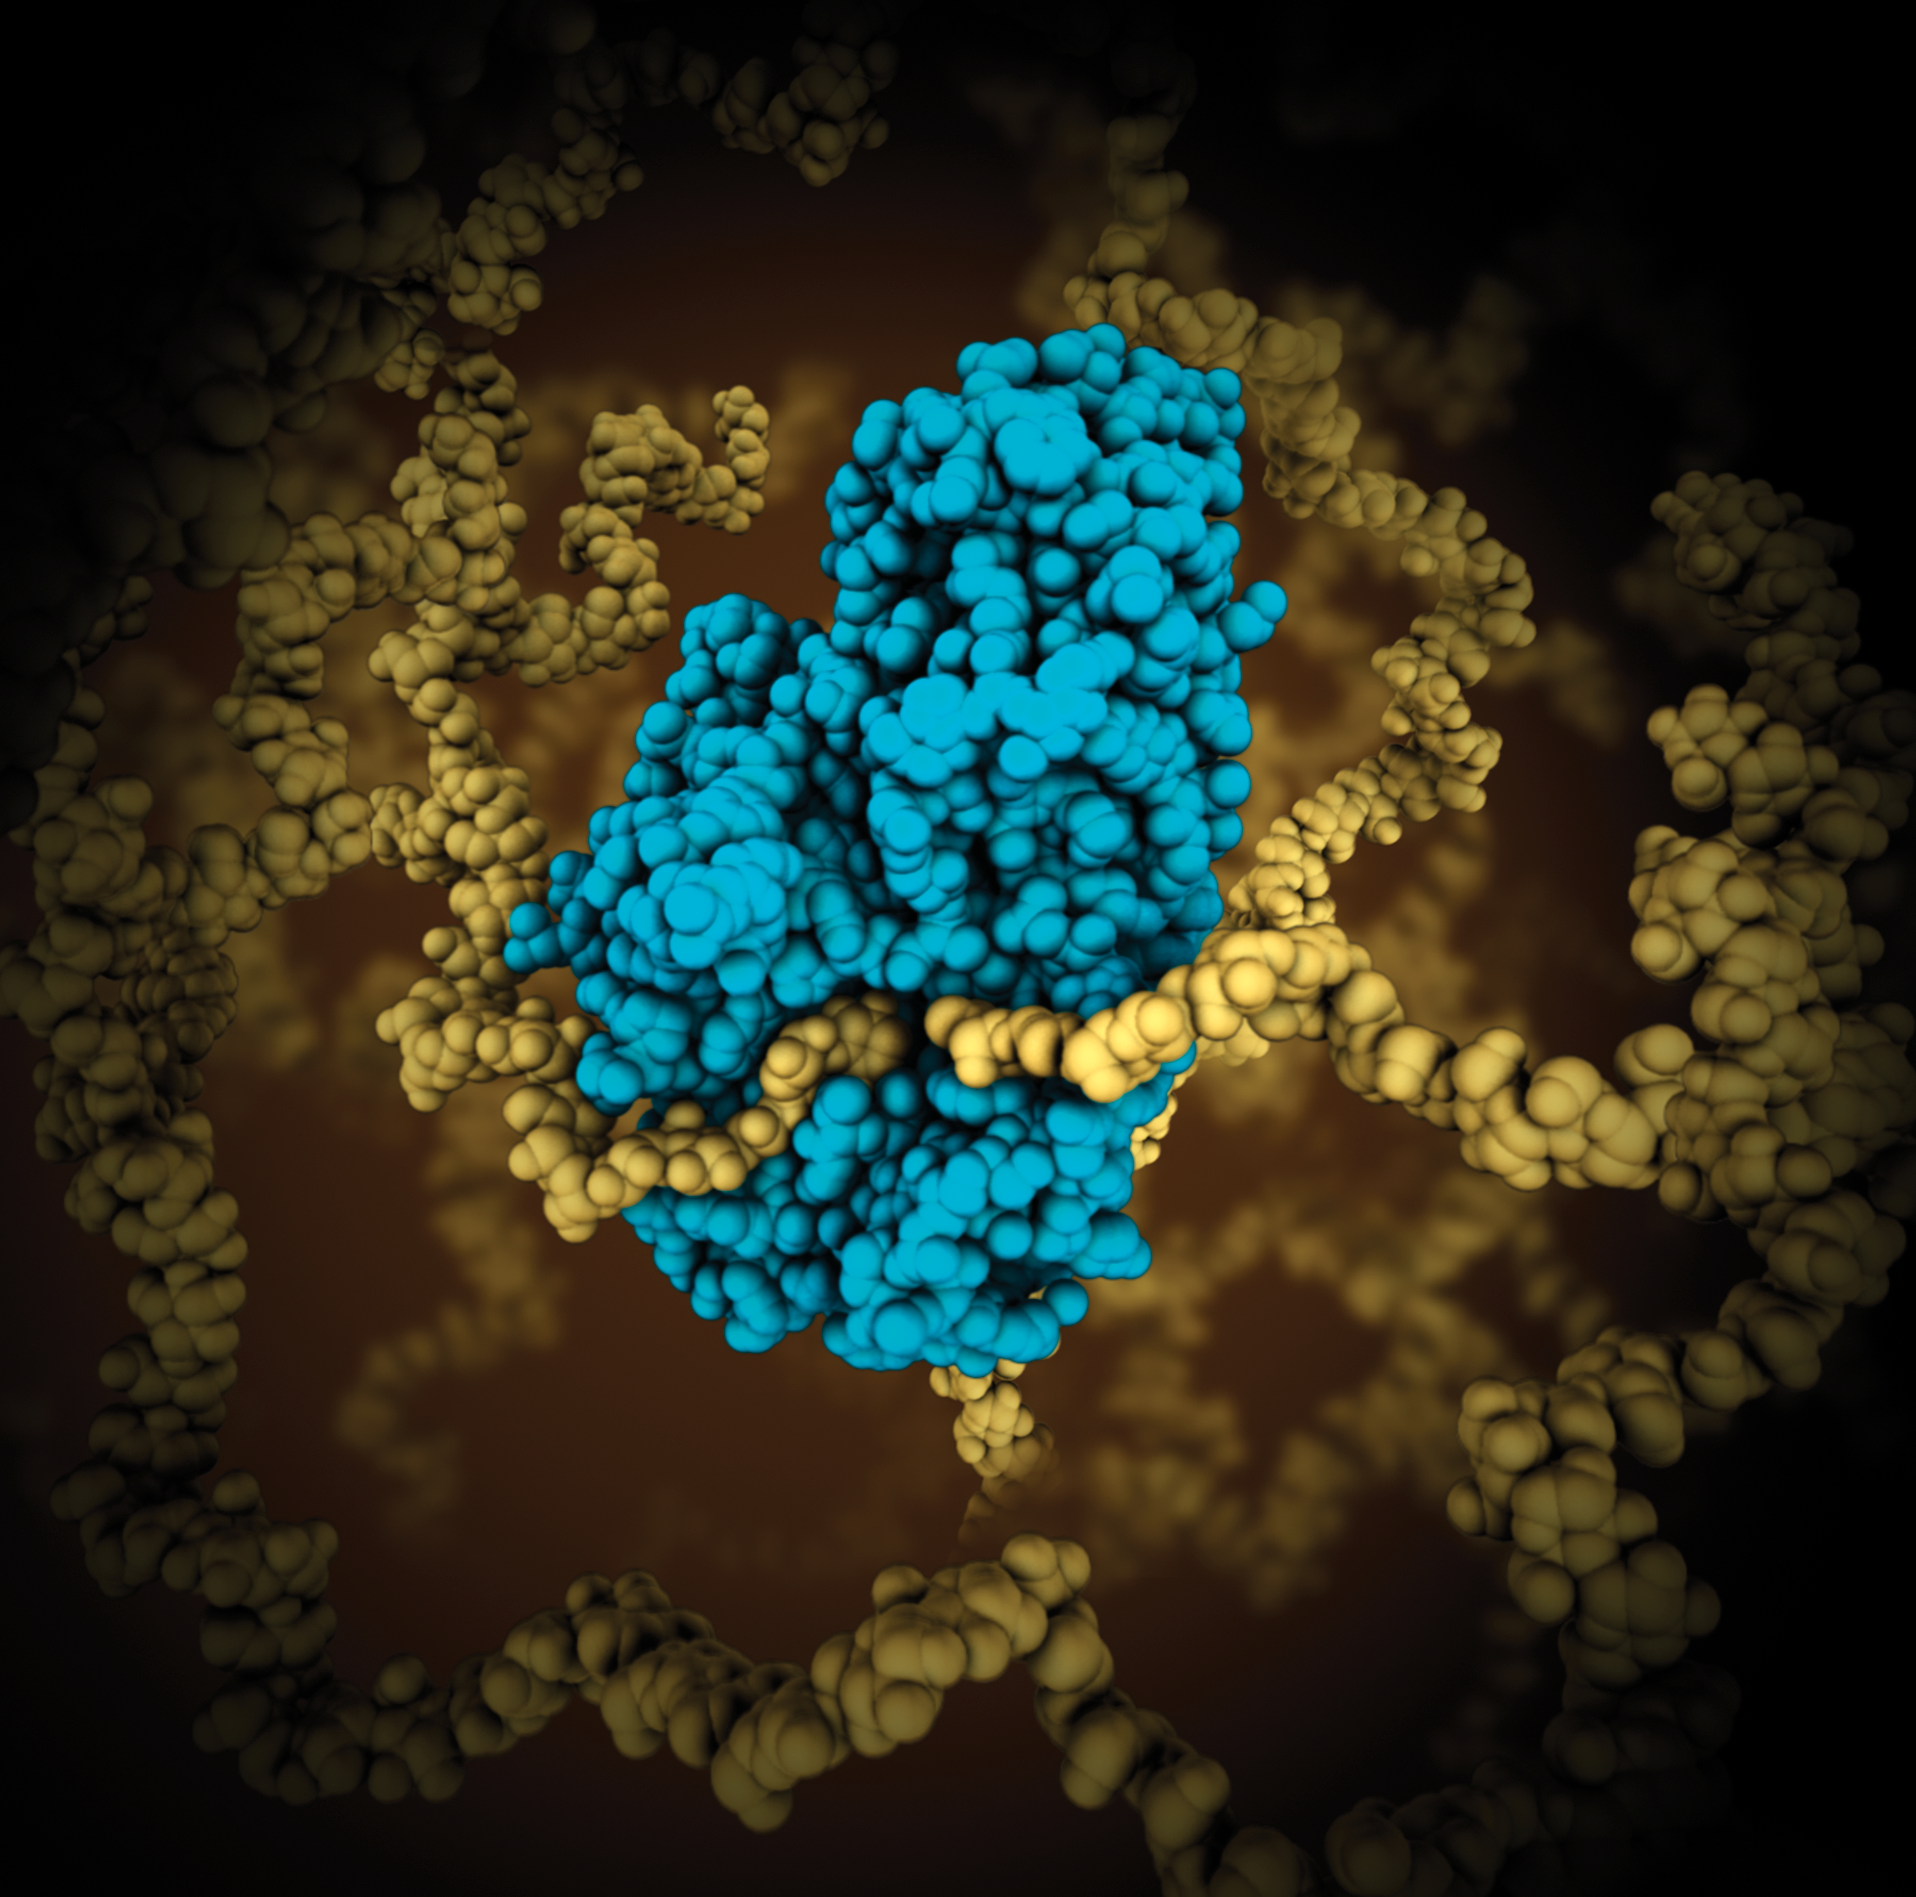
\includegraphics[scale=0.11]{images/Alpha-amylase.png}
	\caption{Enzima alpha Amilasi in turchese, rappresentazione di tipo space-filling. Si lega a catene di carboidrati (gialle) e le rompe in pezzi più piccoli di glucosio. Fonte \cite{ProteinRCSB}}
	\label{fig:amilasi}
	\endminipage\hfill
\end{figure}


Nelle cellule le proteine svolgono, fra le altre, funzioni di supporto strutturale (\textit{collagene}), mobilità (\textit{actina, miosina}), protezione (\textit{anticorpi}), regolazione, ormoni (\textit{insulina}), trasporto, catalisi, magazzino. Nel nostro corpo abbiamo un numero grandissimo di proteine: $10^{27}$. Per usare una metafora di Ken Dill \supercite{TalksDill2013Oct} potremmo dire che se si potesse ingrandire una proteina alla grandezza di un penny (diametro di 19mm) il numero di proteine che una persona ha nel corpo equivale al numero di penny che riempirebbero l'Oceano Pacifico.

\par Per queste e altre ragioni queste macromolecole sono il target di grandi attività di ricerca e di applicazione biotecnologiche: dal combattere malattie infettive \supercite{batool2019structure} al contrastare l'inquinamento ambientale \supercite{knott2020characterization}.

\section{Background informatico}

\subsection{Bioinformatica}

La \textit{bioinformatica} ha giocato un ruolo fondamentale durante l'epidemia di COVID-19, in particolare nella realizzazione di vaccini grazie agli avanzamenti nelle tecnologie NGS (Next Generation Sequencing). La bioinformatica è una disciplina dedicata alla risoluzione di problemi biologici a livello molecolare con metodi informatici, per questa ragione viene anche chiamata \textit{biologia computazionale}. Argomenti di interesse di questa disciplina sono:
\begin{itemize}
	\item allineamento di sequenze genetiche
	\item predizione genica
	\item predizione della struttura di proteine
	\item espressione genica
	\item interazione proteina-proteina
	\item interpretazione di dati proveniente da esperimenti biochimici
	\item organizzazione e archiviazione conoscenze su genomi e proteomi
	\item modellizzazione di sistemi e reti biologiche
\end{itemize}

\par Come si può notare da questa lista una parte importante della bioinformatica si occupa dell'utilizzo di strumenti informatici finalizzati a manipolare, archiviare e confrontare stringhe e sequenze di caratteri. Tuttavia questa disciplina non si ferma all’analisi delle sequenze. Tra le più interessanti applicazioni bioinformatiche odierne vi sono quelle incentrate sull’analisi strutturale \supercite{baxevanis2020bioinformatics}. Difatti la bioinformatica pone le sue fondamenta nel campo della \textit{structural bioinformatics}: per portare un esempio il database PDB (\textit{Protein Data Bank}) nasce nel 1977 per archiviare coordinate atomiche e legami derivati dagli studi cristallografici sulle proteine \supercite{bernstein77}.

\par Non va confusa la bioinformatica (o biologia computazionale) con la \textit{computazione bio-ispirata} (es. algoritmi genetici, reti neurali), con il \textit{biological computing} (ossia computer composti di parti biologiche come DNA, proteine o neuroni) o con la \textit{biological computation} (l'idea che gli organismi eseguano computazioni e che le idee di informazione e computazione possano essere la chiave per comprendere la biologia)\supercite{Mitchell2010}.

\par Il Machine Learning (ML) è uno dei paradigmi informatici che più sta influenzando il campo della bioinformatica (come la presente tesi può dimostrare). Questo è dovuto principalmente a due fattori evolutisi in parallelo negli ultimi anni: la crescita esponenziale di dataset biologici disponibili e i progressi informatici del ML. Gli strumenti di ML possono apprendere caratteristiche dei sistemi biologici inferendole direttamente dai dataset. Quando propriamente allenati questi sistemi possono fornire accurate predizioni di caratteristiche astratte, proprio come nel caso di AlphaFold per il problema della predizione della struttura di proteine.

\subsection{Soft computing}
Il \textit{soft computing} è un paradigma che si contrappone a quello dell'\textit{hard computing}, ovvero la risoluzione di un problema tramite l'esecuzione di un algoritmo ben definito e decidibile. Il soft computing accantona la precisione od ottimalità e innalza a obiettivo il guadagno nella comprensione del comportamento di un sistema. Il soft computing si basa su due principi: 
\begin{enumerate}
	\item l'apprendimento a partire dai dati
	\item l'integrazione di conoscenza umana basata sull'esperienza, strutturata e preesistente, all'interno di modelli matematici computabili
\end{enumerate}

Il ML si avvale delle tecniche del soft computing \supercite{MLwiki} e vi entra pienamente: la stima di performance in ML è infatti l'\textit{accuratezza predittiva}, stimata dall'errore calcolato sul test set.

\begin{figure}[!h]
	\centering
	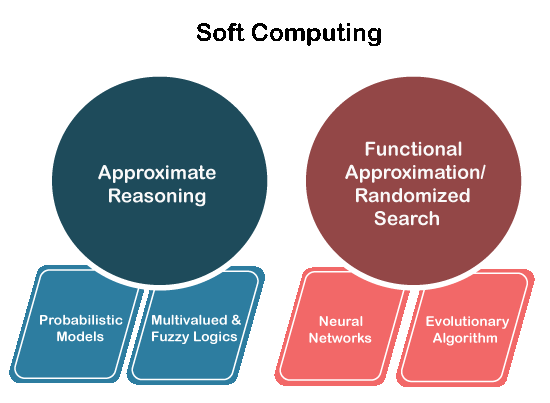
\includegraphics[scale=0.4]{images/soft-computing.png}
	\caption{Branche del soft computing. Fonte: \cite{softComputing}}
	\label{fig:soft-computing}
\end{figure}

\subsubsection{Algoritmi genetici}

\par Gli algoritmi genetici fanno parte del paradigma relativo alle tecniche informatiche \textit{bio-ispirate}, così come le reti neurali. Un algoritmo genetico è un algoritmo euristico utilizzato per tentare di risolvere problemi di ottimizzazione. L'aggettivo "genetico", ispirato al principio della selezione naturale ed evoluzione biologica, deriva dal fatto che, al pari del modello evolutivo darwiniano che trova spiegazioni nella genetica, gli algoritmi genetici attuano dei meccanismi concettualmente simili a quelli dei processi biochimici genetici, come il \textit{crossing over}.

\subsection{Intelligenza Artificiale}

Definire cosa sia l'intelligenza non è un compito semplice. Una definizione ampia e utilizzata nel mondo dell'AI è quella data da Kurzweil:

\say{\textit{L’arte di creare macchine che svolgono funzioni che richiedono intelligenza quando svolte da esseri umani}}\footnote{\fullcite{kurzweil1990age}} \\

Una definizione di intelligenza proveniente da uno sfondo culturale del tutto diverso è la seguente:

\say{\textit{The role of intelligence is to determine the positive and negative potential of an event or factor which could have both positive and negative results. It is the role of intelligence, with the full awareness that is provided by education, to judge and accordingly utilize the potential for one's own benefit or well-being}}\footnote{\fullcite{dalaiLama}} \\

Nella sua accezione più semplice, l'Intelligenza Artificiale (AI) si riferisce a sistemi che imitano l'intelligenza umana per eseguire certe attività e che sono in grado di migliorarsi continuamente in base alle informazioni raccolte. L'IA si occupa della costruzione di macchine intelligenti, della comprensione mediante modelli computazionali dei comportamenti e della psicologia di uomini, animali e agenti artificiali e può avere applicazioni innumerevoli nella società. I fondamenti dell'IA sono sin dalla nascita interdisciplinari: filosofia, matematica, economia, neuroscienze, psicologia, informatica, linguistica, cibernetica, statistica, complessità, teoria del controllo, teoria dell'informazione, robotica.

\begin{figure}[!h]
	\centering
	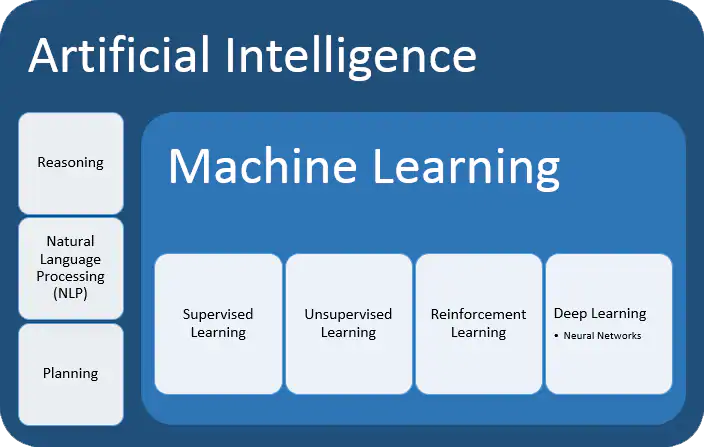
\includegraphics[scale=0.4]{images/artificial-intelligence.png}
	\caption{Schema riassuntivo dei campi dell'IA. Fonte: \cite{ML_IBM}}
	\label{fig:ai}
\end{figure}

\subsection{Machine Learning}

Il Machine Learning (ML) è un sottoinsieme dell'AI che si occupa di creare sistemi che automaticamente migliorano con l'esperienza, basandosi su rigorosi fondamenti delle scienze computazionali. Utilizza metodi statistici per migliorare la performance di un algoritmo nell'identificare pattern nei dati. Domande fondamentali di questo campo sono del tipo: "come varia la performance di apprendimento al variare del numero di esempi di allenamento presentati?". 

\par L'apprendimento è al cuore del problema dell'intelligenza sia biologica che artificiale ed è un principio universale comune a tutti gli organismi. Tom M. Mitchell definisce in questo modo l'apprendimento per una macchina:

\say{\textit{Si dice che un programma apprende dall'esperienza E con riferimento ad alcune classi di compiti T e con misurazione della performance P, se le sue performance nel compito T, come misurato da P, migliorano con l'esperienza E.}}\footnote{\fullcite{mitchell1997machine}} \\

Il ML si divide in:

\begin{itemize}
	\item \textit{Supervised Learning}, ad es. SVM (support vector machine), in cui al modello vengono forniti degli esempi nella forma di possibili input e i rispettivi output desiderati e l'obiettivo è quello di estrarre una regola generale che associ l'input all'output corretto; comuni sono i task di classificazione e regressione \\
	
	\item \textit{Unsupervised Learning}, in cui il modello ha lo scopo di trovare una struttura negli input forniti, come un raggruppamento naturale nei dati, senza che gli input vengano etichettati in alcun modo \\
	
	\item \textit{Reinforcement Learning}, il modello interagisce con un ambiente dinamico nel quale cerca di raggiungere un obiettivo (per esempio guidare un veicolo, o imparare a giocare contro un avversario), avendo un insegnante che gli dice solo se ha raggiunto l'obiettivo \\
	
	\item \textit{Deep Learning}, insieme di tecniche basate su reti neurali artificiali organizzate in diversi strati, dove ogni strato calcola i valori per quello successivo; si basa su diversi livelli di rappresentazione, corrispondenti a gerarchie di caratteristiche
\end{itemize}

Il ML è quindi sì uno strumento molto potente ma è importante comprenderne i limiti. È utile quando non esiste o è difficile da formalizzare la teoria attorno ad un problema, oppure quando i dati da analizzare sono incerti, rumorosi o incompleti.

\subsection{Reti neurali artificiali (ANN)}

Una rete neurale artificiale (\textit{Artificial Neural Network}) è un modello computazionale composto da neuroni artificiali bio-ispirato alla semplificazione di una rete neurale biologica. È importante notare che l'obiettivo della modellizzazione bio-ispirata non è una comprensione delle reti neurali biologiche, data la semplicità dei modelli utilizzati, ma il tentativo di risolvere problemi ingegneristici sfruttando idee derivanti da queste. Nonostante ciò le ANN riflettono tratti di comportamento del cervello umano e consentono di riconoscere pattern e risolvere problemi difficili.

\begin{figure}[!h]
	\centering
	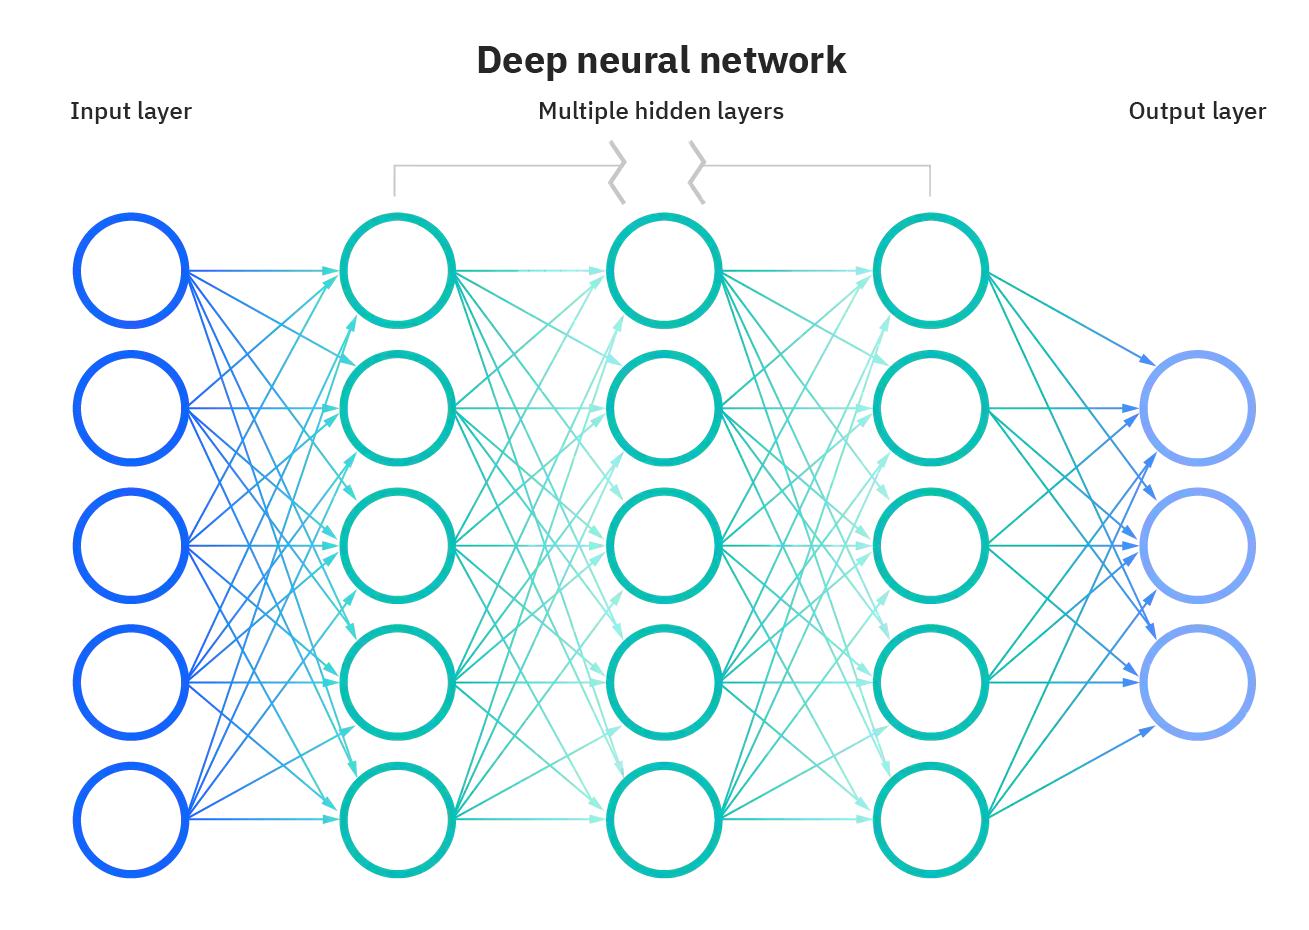
\includegraphics[scale=0.2]{images/ann.png}
	\caption{Rete neurale artificiale. Fonte: \cite{neuralNetworksIBM}}
	\label{fig:rete-neurale}
\end{figure}

\par Le ANN sono composte da strati di nodi: uno strato di input, uno o più nascosti e uno di output. Ogni nodo è un neurone artificiale, si connette a tutti i nodi dello strato successivo e ha associato un peso e una soglia. Se l'output di un nodo è sopra la soglia allora il neurone è attivato, trasferendo informazioni al prossimo strato della rete. Con l'allenamento le ANN possono migliorare la loro accuratezza e rivelarsi potenti strumenti. Campi di utilizzo sono, fra gli altri, lo \textit{speech-recognition} e l'\textit{image recognition}.

\par La parola "deep" in \textit{deep learning} si riferisce alla profondità degli strati in una rete neurale. Una rete neurale artificiale che consiste in almeno 4 strati (inclusi quello di input e output) può essere considerata un algoritmo di \textit{deep learning}\supercite{neuralNetworksIBM}. Una rete neurale con 2 o 3 strati è una rete neurale semplice.

\clearpage